% =====================================================================
%  Chapter 5: Vector-Valued Functions and Motion
%  Drafted to follow the Chapter 5 outline and continue the Chapter 4
%  ending hook: curves now become motion. :contentReference[oaicite:0]{index=0} :contentReference[oaicite:1]{index=1}
% =====================================================================

\chapter{Vector-Valued Functions and Motion}
\label{ch:5}

Chapter 4 taught us how to describe curves before doing calculus on them.  A curve was
a moving point
\[
    \mathbf r(t).
\]
Sometimes \(t\) was only a convenient parameter.  Now \(t\) becomes time.

That small change brings single-variable calculus back into the story.  If
\[
    \mathbf r(t)
\]
records the position of a moving object, then the change in \(\mathbf r\) over a short
time measures velocity.  The change in velocity measures acceleration.  We are about
to differentiate and integrate curves.

\section{Vector-valued functions}
\label{sec:5.1}

Chapter 4 used parametric curves to describe shapes.  The circle
\[
    \mathbf r(t)=(3\cos t,3\sin t)
\]
was a set of points traced by a moving point.  Now we read the same notation in a more
physical way: at time \(t\), where is the object?

A function like this has one input, but its output is a vector.  That is why it is called
a vector-valued function.

\subsection{Position as a function of time}

Imagine a firefly circling a porch light while slowly rising.  Put the light at the origin
of the \(xy\)-plane, and measure height by \(z\).  Suppose the firefly's position at time
\(t\) is
\[
    \mathbf r(t)=\left(2\cos t,\;2\sin t,\;1+\frac{t}{4}\right),
    \qquad 0\le t\le 4\pi.
\]
At a few times,
\[
\begin{array}{c|c}
t & \mathbf r(t) \\ \hline
0 & (2,0,1)\\[1mm]
\dfrac{\pi}{2} & \left(0,2,1+\dfrac{\pi}{8}\right)\\[2mm]
\pi & \left(-2,0,1+\dfrac{\pi}{4}\right)\\[2mm]
2\pi & \left(2,0,1+\dfrac{\pi}{2}\right)
\end{array}
\]
The \(x\)- and \(y\)-coordinates circle around the light.  The \(z\)-coordinate rises
steadily.  The path is a helix.
\begin{figure}[h]
\centering
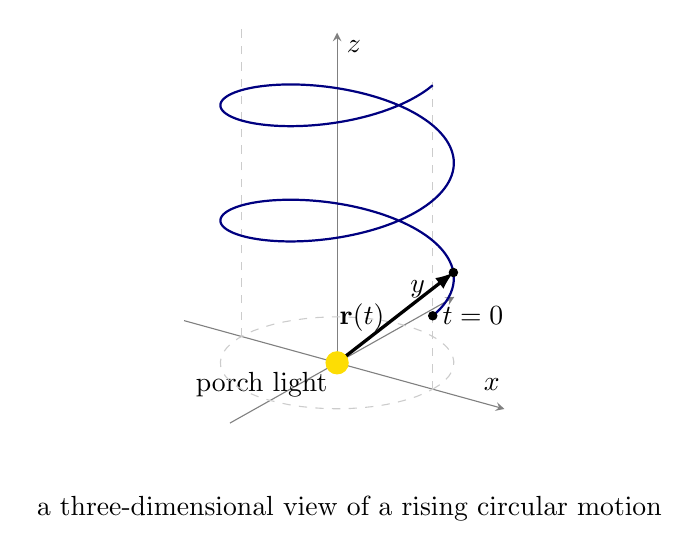
\begin{tikzpicture}[>=latex]

    \begin{axis}[
        name=helixplot,
        view={35}{25},
        width=8.5cm, height=8.5cm,
        axis lines=center,
        axis line style={gray, thin},
        xlabel={\(x\)}, ylabel={\(y\)}, zlabel={\(z\)},
        ticks=none,
        xmin=-3.2, xmax=3.5,
        ymin=-3.2, ymax=3.5,
        zmin=0, zmax=4.5,
    ]

        % Porch light at origin
        \addplot3[only marks, mark=*, mark size=4pt, yellow!80!orange] coordinates {(0,0,0)};
        \node[below left] at (0,0,0) {porch light};

        % Bounding cylinder base for depth perception
        \addplot3[
            gray!40, dashed, 
            domain=0:360, 
            samples=60,
            samples y=0,
            variable=\t
        ] ({2*cos(\t)}, {2*sin(\t)}, 0);
        
        % Vertical bounding lines
        \draw[gray!40, dashed] (2,0,0) -- (2,0,4.2);
        \draw[gray!40, dashed] (-2,0,0) -- (-2,0,4.2);

        % 3D Helix (Firefly path)
        % 2 full turns = 720 degrees. z = 1 + t/(4 rad) -> 1 + (\t * pi / 180) / 4
        \addplot3[
            thick, blue!50!black,
            domain=0:720,
            samples=200,
            samples y=0,
            variable=\t,
            smooth
        ] ({2*cos(\t)}, {2*sin(\t)}, {1 + \t*pi/720});

        % Mark t=0
        \addplot3[only marks, mark=*, mark size=1.5pt] coordinates {(2,0,1)};
        \node[right] at (2,0,1) {\(t=0\)};

        % True position vector r(t) from the origin pointing to t=0.7 radians
        \draw[->, very thick] (0,0,0) -- ({2*cos(deg(0.7))}, {2*sin(deg(0.7))}, {1 + 0.7/4}) 
            node[midway, left] {\(\mathbf{r}(t)\)};
        \addplot3[only marks, mark=*, mark size=1.5pt] coordinates {({2*cos(deg(0.7))}, {2*sin(deg(0.7))}, {1 + 0.7/4})};

    \end{axis}
    
    % Label below
    \node[align=center] at ([yshift=-0.5cm]helixplot.south) {a three-dimensional view of a rising circular motion};

\end{tikzpicture}
\caption{A vector-valued function can record the position of a moving point.}
\end{figure}

The input \(t\) is a number.  The output
\[
    \mathbf r(t)
\]
is a vector in \(\mathbb R^3\).  So this is not a real-valued function like
\[
    f(t)=t^2.
\]
It is a function whose values are vectors.

\begin{definition}[Vector-valued function]
A \emph{vector-valued function} is a function whose output is a vector.

A vector-valued function into \(\mathbb R^n\) has the form
\[
    \mathbf r(t)=\bigl(r_1(t),r_2(t),\ldots,r_n(t)\bigr),
\]
where each \(r_i(t)\) is an ordinary real-valued function.

When \(\mathbf r(t)\) describes motion, we call \(\mathbf r(t)\) the \emph{position vector}
at time \(t\).
\end{definition}

For plane motion,
\[
    \mathbf r(t)=(x(t),y(t)).
\]
For space motion,
\[
    \mathbf r(t)=(x(t),y(t),z(t)).
\]

The coordinate functions
\[
    x(t),\qquad y(t),\qquad z(t)
\]
are called the \emph{component functions}.  They are ordinary single-variable functions,
so the tools of single-variable calculus can act on them.

\subsection{Component functions}

A bird flying through a room might have position
\[
    \mathbf r(t)=(3+t,\;2+\sin t,\;5-\cos t).
\]
This one vector equation is really three equations:
\[
    x(t)=3+t,
\]
\[
    y(t)=2+\sin t,
\]
and
\[
    z(t)=5-\cos t.
\]
Each coordinate tells a different part of the motion.  The \(x\)-coordinate increases
steadily.  The \(y\)-coordinate oscillates.  The \(z\)-coordinate also oscillates, but with
a different timing.

\begin{example}[Reading a motion component by component]
Let
\[
    \mathbf r(t)=(4\cos t,\;4\sin t,\;2t),
    \qquad 0\le t\le 2\pi.
\]
Then
\[
    x(t)=4\cos t,\qquad y(t)=4\sin t,\qquad z(t)=2t.
\]
The first two coordinates keep the point on the cylinder
\[
    x^2+y^2=16.
\]
The third coordinate rises from \(0\) to \(4\pi\).  So the image is one turn of a helix
on a cylinder of radius \(4\).
\end{example}

This way of reading a vector-valued function is simple, but important.  Almost every
calculus operation in this chapter will happen component by component.

\subsection{Limits of vector-valued functions}

A moving object has a limiting position as \(t\) approaches \(a\) if its whole position
settles down to one vector.

For example, consider
\[
    \mathbf r(t)=
    \left(
        \frac{t^2-1}{t-1},\;
        \sin(\pi t),\;
        \sqrt{t+3}
    \right),
    \qquad t\ne 1.
\]
The formula is not defined at \(t=1\), because the first component contains
\[
    \frac{t^2-1}{t-1}.
\]
But for \(t\ne1\),
\[
    \frac{t^2-1}{t-1}
    =
    \frac{(t-1)(t+1)}{t-1}
    =
    t+1.
\]
So as \(t\to1\),
\[
    \frac{t^2-1}{t-1}\to2,
\]
\[
    \sin(\pi t)\to \sin\pi=0,
\]
and
\[
    \sqrt{t+3}\to2.
\]
Therefore
\[
    \lim_{t\to1}\mathbf r(t)=(2,0,2).
\]

\begin{definition}[Limit of a vector-valued function]
We write
\[
    \lim_{t\to a}\mathbf r(t)=\mathbf L
\]
if the distance
\[
    \|\mathbf r(t)-\mathbf L\|
\]
approaches \(0\) as \(t\) approaches \(a\).
\end{definition}

The definition says exactly what it should say: the vector \(\mathbf r(t)\) gets close to
\(\mathbf L\) if the distance between them gets small.

The previous example suggests the main rule.

\begin{theorem}[Limits are componentwise]
Let
\[
    \mathbf r(t)=\bigl(r_1(t),r_2(t),\ldots,r_n(t)\bigr)
\]
and
\[
    \mathbf L=(L_1,L_2,\ldots,L_n).
\]
Then
\[
    \lim_{t\to a}\mathbf r(t)=\mathbf L
\]
if and only if
\[
    \lim_{t\to a}r_i(t)=L_i
\]
for every component \(i=1,2,\ldots,n\).
\end{theorem}

\begin{proof}
The distance from \(\mathbf r(t)\) to \(\mathbf L\) is
\[
    \|\mathbf r(t)-\mathbf L\|
    =
    \sqrt{
    (r_1(t)-L_1)^2+\cdots+(r_n(t)-L_n)^2
    }.
\]
If this distance goes to \(0\), then each component difference must go to \(0\).

Conversely, if every component difference goes to \(0\), then the sum of their squares
goes to \(0\), so the square root also goes to \(0\).  Thus the whole vector approaches
\(\mathbf L\).
\end{proof}

We really do need every component to settle down.

\begin{example}[One bad component breaks the limit]
Define
\[
    \mathbf r(t)=\left(t,\sin\frac{1}{t}\right),
    \qquad t\ne0.
\]
The first component has a limit:
\[
    t\to0.
\]
But the second component
\[
    \sin\frac{1}{t}
\]
oscillates forever as \(t\to0\).  It does not approach one number.

So the vector-valued function has no limit at \(t=0\).  The first coordinate behaves
well, but the whole point does not settle down.
\end{example}

This is the same lesson as in single-variable calculus, but now it can fail in any
coordinate.

\subsection{Continuity}

A position function is continuous when the moving point does not jump.

\begin{definition}[Continuity of a vector-valued function]
A vector-valued function \(\mathbf r(t)\) is \emph{continuous at \(a\)} if
\[
    \lim_{t\to a}\mathbf r(t)=\mathbf r(a).
\]
It is continuous on an interval if it is continuous at every point of that interval
with the usual one-sided interpretation at endpoints.
\end{definition}

By the componentwise limit theorem, continuity is also componentwise.

\begin{theorem}[Continuity is componentwise]
The vector-valued function
\[
    \mathbf r(t)=\bigl(r_1(t),r_2(t),\ldots,r_n(t)\bigr)
\]
is continuous at \(a\) if and only if each component function \(r_i(t)\) is continuous
at \(a\).
\end{theorem}

\begin{example}[A continuous motion]
The function
\[
    \mathbf r(t)=(\cos t,\sin t,t)
\]
is continuous for every \(t\), because \(\cos t\), \(\sin t\), and \(t\) are continuous.
The curve is a helix with no jumps.
\end{example}

Here is why the continuity condition matters.

\begin{example}[A jump is not a curve of steady motion]
Define
\[
    \mathbf r(t)=
    \begin{cases}
    (t,0), & t<0,\\
    (t,1), & t\ge0.
    \end{cases}
\]
For \(t<0\), the point moves along the line \(y=0\).  For \(t\ge0\), it moves along
the line \(y=1\).

At \(t=0\),
\[
    \mathbf r(0)=(0,1).
\]
But as \(t\to0^-\),
\[
    \mathbf r(t)\to(0,0).
\]
The left-hand limiting position and the actual position at \(0\) do not agree.  The
point teleports upward.

So this function is not continuous at \(t=0\).
\end{example}

A curve used to model physical motion is usually continuous.  Later, when we want
velocity, we will ask for more: differentiability.

\subsection{Space curves as images of intervals}

The \emph{image} of a vector-valued function
\[
    \mathbf r:I\to\mathbb R^n
\]
is the set of all points reached:
\[
    \{\mathbf r(t):t\in I\}.
\]
This image is the geometric curve.  But the function \(\mathbf r(t)\) contains more
information than the image alone.

\begin{example}[The same image with different clocks]
The two functions
\[
    \mathbf r_1(t)=(\cos t,\sin t),
    \qquad 0\le t\le2\pi,
\]
and
\[
    \mathbf r_2(s)=(\cos 2s,\sin 2s),
    \qquad 0\le s\le\pi,
\]
have the same image: the unit circle.

But the clocks are different.  In \(\mathbf r_1\), the angle is \(t\).  In \(\mathbf r_2\),
the angle is \(2s\).  The second parametrization moves around the circle twice as fast
with respect to its parameter.
\end{example}

\begin{example}[The same circle traced twice]
The function
\[
    \mathbf r(t)=(\cos t,\sin t),
    \qquad 0\le t\le4\pi,
\]
also has the unit circle as its image.  But it traces the circle twice.

The image does not remember how many times the curve is traced.  The parametrization
does.
\end{example}

This distinction will matter whenever we integrate along a curve.  If we walk around a
circle twice, an accumulated quantity may be twice as large.  If we reverse direction,
some accumulated quantities change sign.

In the language of differentials, the components of a curve also tell us how \(dx\),
\(dy\), and \(dz\) change along the curve.  If
\[
    x=x(t),
\]
then later we will write
\[
    dx=x'(t)\,dt.
\]
That is the first hint of how a \(1\)-form like
\[
    P\,dx+Q\,dy+R\,dz
\]
will be pulled back to an ordinary one-variable integral along a path.

For now, a vector-valued function gives us a position record.  The next question is the
one every motion problem asks first: how fast is the position changing?

\section{Derivatives and integrals of vector-valued functions}
\label{sec:5.2}

Section \ref{sec:5.1} made \(\mathbf r(t)\) a position record.  A position record becomes
useful when we compare nearby times.  The difference
\[
    \mathbf r(t+h)-\mathbf r(t)
\]
is a displacement.  Dividing by \(h\) gives average velocity over a short time interval.

Then the old single-variable idea returns: let the time interval shrink.

\subsection{Velocity from a difference quotient}

A small drone flies through a warehouse.  Its position, in meters, is
\[
    \mathbf r(t)=\left(t,\;t^2,\;3-\frac{t}{2}\right),
\]
where \(t\) is measured in seconds.

At \(t=1\),
\[
    \mathbf r(1)=\left(1,1,\frac52\right).
\]
At time \(1+h\),
\[
    \mathbf r(1+h)=
    \left(1+h,\;(1+h)^2,\;3-\frac{1+h}{2}\right).
\]
The displacement from \(t=1\) to \(t=1+h\) is
\[
\begin{aligned}
    \mathbf r(1+h)-\mathbf r(1)
    &=
    \left(
        h,\;
        (1+h)^2-1,\;
        -\frac{h}{2}
    \right)\\
    &=
    \left(
        h,\;
        2h+h^2,\;
        -\frac{h}{2}
    \right).
\end{aligned}
\]
The average velocity over that interval is
\[
\frac{\mathbf r(1+h)-\mathbf r(1)}{h}
=
\left(
    1,\;
    2+h,\;
    -\frac12
\right).
\]
Letting \(h\to0\), we get the instantaneous velocity at \(t=1\):
\[
    \left(1,2,-\frac12\right).
\]

This vector points in the direction the drone is moving at that instant.

\begin{definition}[Derivative of a vector-valued function]
The derivative of
\[
    \mathbf r(t)
\]
at \(t=a\) is
\[
\boxed{
    \mathbf r'(a)=
    \lim_{h\to0}
    \frac{\mathbf r(a+h)-\mathbf r(a)}{h}
}
\]
when this limit exists.
\end{definition}

When \(\mathbf r(t)\) is a position vector, the derivative
\[
    \mathbf v(t)=\mathbf r'(t)
\]
is called the \emph{velocity}.  The derivative of velocity,
\[
    \mathbf a(t)=\mathbf v'(t)=\mathbf r''(t),
\]
is called the \emph{acceleration}.

For the drone,
\[
    \mathbf r(t)=\left(t,\;t^2,\;3-\frac{t}{2}\right),
\]
so we expect
\[
    \mathbf v(t)=\left(1,2t,-\frac12\right),
\]
and
\[
    \mathbf a(t)=(0,2,0).
\]
We will justify the component-by-component rule next.

\subsection{Differentiating component by component}

A helix gives a clean example.  Let
\[
    \mathbf r(t)=\left(2\cos t,\;2\sin t,\;\frac{t}{3}\right).
\]
The component functions are
\[
    x(t)=2\cos t,\qquad y(t)=2\sin t,\qquad z(t)=\frac{t}{3}.
\]
Differentiating each one gives
\[
    x'(t)=-2\sin t,
\]
\[
    y'(t)=2\cos t,
\]
and
\[
    z'(t)=\frac13.
\]
So
\[
    \mathbf r'(t)=\left(-2\sin t,\;2\cos t,\;\frac13\right).
\]
At \(t=0\),
\[
    \mathbf r(0)=(2,0,0),
\]
and
\[
    \mathbf r'(0)=\left(0,2,\frac13\right).
\]
The point is at the right side of the circle and is moving in the positive \(y\)-direction
while also rising.

\begin{figure}[h]
\centering
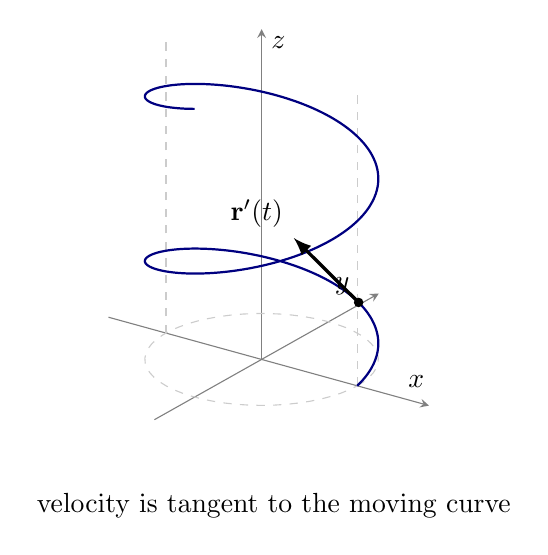
\begin{tikzpicture}[>=latex]

    \begin{axis}[
        name=helixplot,
        view={35}{25},
        width=8.5cm, height=8.5cm,
        axis lines=center,
        axis line style={gray, thin},
        xlabel={\(x\)}, ylabel={\(y\)}, zlabel={\(z\)},
        ticks=none,
        xmin=-3.2, xmax=3.5,
        ymin=-3.2, ymax=3.5,
        zmin=0, zmax=4.2,
    ]

        % Bounding cylinder base for depth perception
        \addplot3[
            gray!40, dashed, 
            domain=0:360, 
            samples=60,
            samples y=0,
            variable=\t
        ] ({2*cos(\t)}, {2*sin(\t)}, 0);
        
        % Vertical bounding lines
        \draw[gray!40, dashed] (2,0,0) -- (2,0,3.8);
        \draw[gray!40, dashed] (-2,0,0) -- (-2,0,3.8);

        % 3D Helix
        % Using the book's function: r(t) = (2 cos t, 2 sin t, t/3)
        % 1.75 turns = 630 degrees. z = t/3 = (\t * pi / 180) / 3 = \t * pi / 540
        \addplot3[
            thick, blue!50!black,
            domain=0:630,
            samples=200,
            samples y=0,
            variable=\t,
            smooth
        ] ({2*cos(\t)}, {2*sin(\t)}, {\t*pi/540});

        % The Point P at t = 1.2 radians
        \addplot3[only marks, mark=*, mark size=1.5pt] 
            coordinates {({2*cos(deg(1.2))}, {2*sin(deg(1.2))}, {1.2/3})};
        
        % True 3D Tangent Vector r'(t) at t = 1.2 radians
        % Tip = P + r'(1.2) = P + (-2 sin(1.2), 2 cos(1.2), 1/3)
        \draw[->, very thick] 
            ({2*cos(deg(1.2))}, {2*sin(deg(1.2))}, {1.2/3}) -- 
            ({2*cos(deg(1.2)) - 2*sin(deg(1.2))}, {2*sin(deg(1.2)) + 2*cos(deg(1.2))}, {1.2/3 + 1/3})
            node[above left] {\(\mathbf{r}'(t)\)};

    \end{axis}
    
    % Label positioned below the axis environment
    \node[align=center] at ([yshift=-0.5cm]helixplot.south) {velocity is tangent to the moving curve};

\end{tikzpicture}
\caption{The derivative vector points tangent to the path.}
\end{figure}

The rule is exactly what the example showed.

\begin{theorem}[Componentwise differentiation]
Let
\[
    \mathbf r(t)=\bigl(r_1(t),r_2(t),\ldots,r_n(t)\bigr).
\]
Then \(\mathbf r'(a)\) exists if and only if each component derivative
\[
    r_i'(a)
\]
exists.  In that case,
\[
\boxed{
    \mathbf r'(a)=
    \bigl(r_1'(a),r_2'(a),\ldots,r_n'(a)\bigr).
}
\]
\end{theorem}

\begin{proof}
Use the definition:
\[
\frac{\mathbf r(a+h)-\mathbf r(a)}{h}
=
\left(
\frac{r_1(a+h)-r_1(a)}{h},
\ldots,
\frac{r_n(a+h)-r_n(a)}{h}
\right).
\]
A vector limit exists exactly when all component limits exist.  Those component limits
are the ordinary derivatives \(r_i'(a)\).
\end{proof}

The hypothesis that the component derivatives exist is real.  A continuous curve can
still fail to have a velocity.

\begin{example}[A sharp corner has no velocity vector]
Let
\[
    \mathbf r(t)=(|t|,t).
\]
This curve is continuous at \(t=0\), but
\[
    \frac{\mathbf r(h)-\mathbf r(0)}{h}
    =
    \left(\frac{|h|}{h},1\right).
\]
If \(h>0\), this quotient is
\[
    (1,1).
\]
If \(h<0\), it is
\[
    (-1,1).
\]
The two one-sided limits do not agree.  Therefore \(\mathbf r'(0)\) does not exist.

Geometrically, the curve has a corner at the origin.  The point arrives from one
direction and leaves in another, so there is no single tangent velocity at that instant.
\end{example}

At endpoints of a time interval, we use the same caution as in single-variable calculus.
A curve defined only for \(t\ge0\) may have a right-hand velocity at \(t=0\), but not a
two-sided derivative there unless the curve is defined on both sides.

\subsection{Tangent lines to a motion path}

If
\[
    \mathbf r'(a)\ne\mathbf 0,
\]
then the tangent line to the curve at time \(a\) is the line through
\[
    \mathbf r(a)
\]
in the direction
\[
    \mathbf r'(a).
\]
Thus
\[
\boxed{
    \mathbf L(s)=\mathbf r(a)+s\mathbf r'(a)
}
\]
is a parametrization of the tangent line.

\begin{example}[A tangent line to a drone path]
For
\[
    \mathbf r(t)=\left(t,\;t^2,\;3-\frac{t}{2}\right),
\]
we found
\[
    \mathbf r(1)=\left(1,1,\frac52\right)
\]
and
\[
    \mathbf r'(1)=\left(1,2,-\frac12\right).
\]
So the tangent line at \(t=1\) is
\[
    \mathbf L(s)
    =
    \left(1,1,\frac52\right)
    +
    s\left(1,2,-\frac12\right).
\]
In coordinates,
\[
    x=1+s,\qquad
    y=1+2s,\qquad
    z=\frac52-\frac{s}{2}.
\]
\end{example}

The velocity vector gives the instantaneous direction of motion, not merely the
direction of the curve as a set.  If the same geometric curve is traced with a different
clock, the velocity vector changes.

\begin{example}[Same circle, different speeds]
Let
\[
    \mathbf r_1(t)=(\cos t,\sin t)
\]
and
\[
    \mathbf r_2(t)=(\cos 2t,\sin 2t).
\]
Both trace the unit circle.  But
\[
    \mathbf r_1'(t)=(-\sin t,\cos t),
\]
while
\[
    \mathbf r_2'(t)=(-2\sin 2t,2\cos 2t).
\]
The second velocity vector has twice the length.  The same circle is being traced twice
as fast.
\end{example}

The length of the velocity vector is the \emph{speed}:
\[
    \text{speed}=\|\mathbf r'(t)\|.
\]
Speed will become the key to arc length in Section \ref{sec:5.3}.

\subsection{Differentiation rules}

Since derivatives are computed component by component, the familiar single-variable
rules return almost unchanged.

Before listing them, here is one example.

\begin{example}[A dot product changing with time]
Let
\[
    \mathbf r(t)=(t,t^2,0),
    \qquad
    \mathbf s(t)=(1,\cos t,\sin t).
\]
Then
\[
    \mathbf r(t)\cdot\mathbf s(t)
    =
    t+t^2\cos t.
\]
Differentiating directly,
\[
    \frac{d}{dt}\bigl(\mathbf r(t)\cdot\mathbf s(t)\bigr)
    =
    1+2t\cos t-t^2\sin t.
\]

Now compute using a product rule:
\[
    \mathbf r'(t)=(1,2t,0),
\]
\[
    \mathbf s'(t)=(0,-\sin t,\cos t).
\]
Then
\[
\begin{aligned}
\mathbf r'(t)\cdot\mathbf s(t)+\mathbf r(t)\cdot\mathbf s'(t)
&=
(1,2t,0)\cdot(1,\cos t,\sin t)\\
&\quad +(t,t^2,0)\cdot(0,-\sin t,\cos t)\\
&=
1+2t\cos t-t^2\sin t.
\end{aligned}
\]
The ordinary product rule is still there, but now it is written with dot products.
\end{example}

\begin{theorem}[Differentiation rules for vector-valued functions]
Suppose \(\mathbf r(t)\) and \(\mathbf s(t)\) are differentiable vector-valued functions,
and \(f(t)\) is a differentiable real-valued function.  Then
\[
    \frac{d}{dt}\bigl(\mathbf r+\mathbf s\bigr)
    =
    \mathbf r'+\mathbf s',
\]
\[
    \frac{d}{dt}\bigl(f\mathbf r\bigr)
    =
    f'\mathbf r+f\mathbf r',
\]
and
\[
    \frac{d}{dt}\bigl(\mathbf r\cdot\mathbf s\bigr)
    =
    \mathbf r'\cdot\mathbf s+\mathbf r\cdot\mathbf s'.
\]
If \(\mathbf r(t)\) and \(\mathbf s(t)\) are functions into \(\mathbb R^3\), then
\[
    \frac{d}{dt}\bigl(\mathbf r\times\mathbf s\bigr)
    =
    \mathbf r'\times\mathbf s+\mathbf r\times\mathbf s'.
\]
\end{theorem}

\begin{proof}
Each rule follows by writing the vectors in components and applying the ordinary
single-variable differentiation rules.  The dot product rule, for example, is just the
product rule applied to each term:
\[
    \mathbf r\cdot\mathbf s
    =
    r_1s_1+\cdots+r_ns_n.
\]
Then
\[
\begin{aligned}
\frac{d}{dt}(\mathbf r\cdot\mathbf s)
&=
(r_1's_1+r_1s_1')+\cdots+(r_n's_n+r_ns_n')\\
&=
\mathbf r'\cdot\mathbf s+\mathbf r\cdot\mathbf s'.
\end{aligned}
\]
The cross product rule is checked the same way from the component formula for
\(\mathbf r\times\mathbf s\).
\end{proof}

The differentiability assumptions matter.  If a component has a corner, as in
\[
    |t|,
\]
then the corresponding vector function may fail to have a derivative, and the rules
above have nothing to apply to at that time.

\subsection{Integrating vector-valued functions}

Differentiation takes us from position to velocity:
\[
    \mathbf r(t)\longmapsto \mathbf r'(t).
\]
Integration goes the other way.  It adds many tiny velocity vectors to recover a net
displacement.

Suppose a drifting boat has velocity
\[
    \mathbf v(t)=(2,\cos t,3t^2),
    \qquad 0\le t\le\pi.
\]
The displacement from \(t=0\) to \(t=\pi\) is
\[
    \int_0^\pi \mathbf v(t)\,dt.
\]
Compute component by component:
\[
\begin{aligned}
\int_0^\pi (2,\cos t,3t^2)\,dt
&=
\left(
    \int_0^\pi 2\,dt,\;
    \int_0^\pi \cos t\,dt,\;
    \int_0^\pi 3t^2\,dt
\right)\\
&=
\left(
    2\pi,\;
    \sin t\bigg|_0^\pi,\;
    t^3\bigg|_0^\pi
\right)\\
&=
(2\pi,0,\pi^3).
\end{aligned}
\]
The boat's net displacement is
\[
    (2\pi,0,\pi^3).
\]

\begin{definition}[Integral of a vector-valued function]
If
\[
    \mathbf v(t)=\bigl(v_1(t),v_2(t),\ldots,v_n(t)\bigr),
\]
then
\[
\boxed{
    \int_a^b \mathbf v(t)\,dt
    =
    \left(
        \int_a^b v_1(t)\,dt,\;
        \int_a^b v_2(t)\,dt,\;
        \ldots,\;
        \int_a^b v_n(t)\,dt
    \right)
}
\]
whenever the component integrals exist.
\end{definition}

For an indefinite integral,
\[
    \int \mathbf v(t)\,dt
\]
means a vector-valued antiderivative:
\[
    \mathbf R'(t)=\mathbf v(t).
\]
The constant of integration is now a constant vector.

\begin{example}[A vector antiderivative]
Let
\[
    \mathbf v(t)=(6t,\;e^t,\;\cos t).
\]
Then
\[
    \int \mathbf v(t)\,dt
    =
    (3t^2,\;e^t,\;\sin t)+\mathbf C,
\]
where
\[
    \mathbf C=(C_1,C_2,C_3)
\]
is a constant vector.
\end{example}

The condition that the component integrals exist is not decoration.  If even one
component fails to have an ordinary definite integral, then the vector integral fails.

\begin{example}[One bad component breaks the vector integral]
The function
\[
    \mathbf v(t)=\left(\frac1t,0\right)
\]
is not bounded near \(t=0\).  The ordinary integral
\[
    \int_0^1 \frac1t\,dt
\]
does not exist as a finite definite integral.  Therefore
\[
    \int_0^1 \left(\frac1t,0\right)\,dt
\]
does not exist as an ordinary vector integral.

A vector integral is only as well behaved as its components.
\end{example}

\subsection{The Fundamental Theorem for vector-valued functions}

The Fundamental Theorem of Calculus now returns in vector form.

\begin{theorem}[Fundamental Theorem for vector-valued functions]
Let
\[
    \mathbf r(t)=\bigl(r_1(t),\ldots,r_n(t)\bigr)
\]
be differentiable on an interval, and suppose \(\mathbf r'(t)\) has continuous
components on \([a,b]\).  Then
\[
\boxed{
    \int_a^b \mathbf r'(t)\,dt
    =
    \mathbf r(b)-\mathbf r(a).
}
\]
\end{theorem}

\begin{proof}
Write
\[
    \mathbf r'(t)=\bigl(r_1'(t),\ldots,r_n'(t)\bigr).
\]
Then
\[
\begin{aligned}
\int_a^b \mathbf r'(t)\,dt
&=
\left(
    \int_a^b r_1'(t)\,dt,\ldots,\int_a^b r_n'(t)\,dt
\right)\\
&=
\left(
    r_1(b)-r_1(a),\ldots,r_n(b)-r_n(a)
\right)\\
&=
\mathbf r(b)-\mathbf r(a).
\end{aligned}
\]
The middle step is the single-variable Fundamental Theorem of Calculus, applied one
component at a time.
\end{proof}

The continuity assumption on the components of \(\mathbf r'\) is a friendly sufficient
condition.  It guarantees that the component integrals behave exactly as expected.  There
are more advanced versions with weaker hypotheses, but this one is the right tool for
the curves in this course.

For motion, the theorem says:
\[
\boxed{
    \int_a^b \mathbf v(t)\,dt
    =
    \mathbf r(b)-\mathbf r(a).
}
\]
The integral of velocity is displacement.

\subsection{Initial value problems for motion}

Often we know velocity or acceleration first, and we want position.

A basketball is thrown across a gym.  Let the \(x\)-axis point across the court, the
\(y\)-axis point sideways, and the \(z\)-axis point upward.  Suppose the ball starts at
\[
    \mathbf r(0)=(0,0,1)
\]
meters and has initial velocity
\[
    \mathbf v(0)=(8,3,10)
\]
meters per second.  Ignore air resistance.  Then acceleration is constant:
\[
    \mathbf a(t)=(0,0,-9.8).
\]

Since
\[
    \mathbf v'(t)=\mathbf a(t),
\]
we integrate acceleration:
\[
    \mathbf v(t)=\int (0,0,-9.8)\,dt
    =
    (0,0,-9.8t)+\mathbf C.
\]
Use
\[
    \mathbf v(0)=(8,3,10)
\]
to get
\[
    \mathbf C=(8,3,10).
\]
Thus
\[
    \mathbf v(t)=(8,3,10-9.8t).
\]

Now integrate velocity:
\[
    \mathbf r(t)=\int (8,3,10-9.8t)\,dt
    =
    (8t,3t,10t-4.9t^2)+\mathbf D.
\]
Use
\[
    \mathbf r(0)=(0,0,1)
\]
to get
\[
    \mathbf D=(0,0,1).
\]
Therefore
\[
\boxed{
    \mathbf r(t)=(8t,\;3t,\;1+10t-4.9t^2).
}
\]

The three coordinates tell three simpler stories:
\[
    x(t)=8t,
\]
\[
    y(t)=3t,
\]
\[
    z(t)=1+10t-4.9t^2.
\]
The horizontal motion is linear.  The vertical motion is the familiar falling-object
parabola from single-variable calculus.

\begin{example}[Recovering position from velocity]
A small underwater robot has velocity
\[
    \mathbf v(t)=(1+t,\;2,\;e^{-t})
\]
and starts at
\[
    \mathbf r(0)=(3,-1,0).
\]
Find \(\mathbf r(t)\).

Since
\[
    \mathbf r'(t)=\mathbf v(t),
\]
we integrate:
\[
    \mathbf r(t)
    =
    \left(
        t+\frac{t^2}{2},\;
        2t,\;
        -e^{-t}
    \right)+\mathbf C.
\]
Use the initial position:
\[
    \mathbf r(0)=(0,0,-1)+\mathbf C=(3,-1,0).
\]
So
\[
    \mathbf C=(3,-1,1).
\]
Therefore
\[
\boxed{
    \mathbf r(t)=
    \left(
        3+t+\frac{t^2}{2},\;
        -1+2t,\;
        1-e^{-t}
    \right).
}
\]
\end{example}

This is an initial value problem.  The derivative information gives a family of possible
motions.  The initial condition chooses the one motion that actually starts in the given
place.

Differentiation and integration now work for motion in space.  But a subtle problem has
appeared.  The integral of velocity gives displacement, not distance traveled.  A runner
who completes one lap has
\[
    \mathbf r(b)-\mathbf r(a)=\mathbf 0,
\]
but she certainly did not run zero meters.  To measure distance traveled, we must add
up tiny lengths
\[
    \|\mathbf r'(t)\|\,dt.
\]
That question leads directly to arc length and speed.

\section{Arc length and speed}
\label{sec:5.3}

Section \ref{sec:5.2} ended with a warning.  The integral of velocity gives
displacement:
\[
    \int_a^b \mathbf r'(t)\,dt=\mathbf r(b)-\mathbf r(a).
\]
But displacement is not the same as distance traveled.  A runner who completes one lap
around a track has returned to the starting point, so the displacement is zero.  The run
was not zero meters long.

\subsection{Distance traveled versus displacement}

Picture a circular track of radius \(50\) meters.  A runner completes one lap in
\(40\) seconds.  A convenient position function is
\[
    \mathbf r(t)=
    \left(
        50\cos\frac{2\pi t}{40},
        50\sin\frac{2\pi t}{40}
    \right),
    \qquad 0\le t\le 40.
\]
At \(t=0\),
\[
    \mathbf r(0)=(50,0).
\]
At \(t=40\),
\[
    \mathbf r(40)=(50,0).
\]
So the displacement is
\[
    \mathbf r(40)-\mathbf r(0)=\mathbf 0.
\]

But the distance traveled is the circumference:
\[
    2\pi(50)=100\pi.
\]
The displacement remembers only the start and finish.  Distance traveled remembers the
whole path.

\begin{figure}[h]
\centering
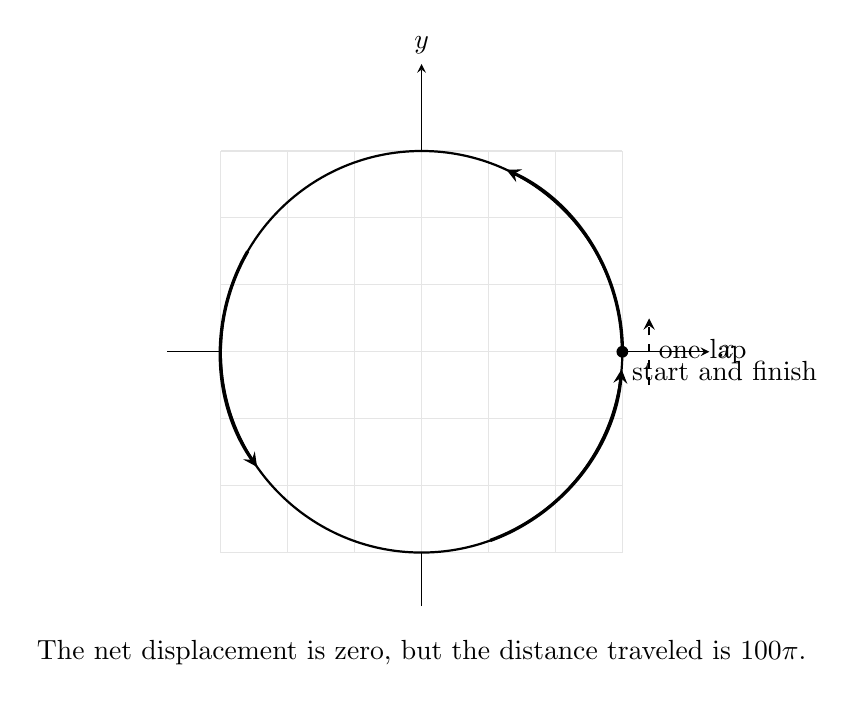
\begin{tikzpicture}[scale=0.85, >=stealth]
    \draw[->] (-3.8,0) -- (4.3,0) node[right] {\(x\)};
    \draw[->] (0,-3.8) -- (0,4.3) node[above] {\(y\)};

    \draw[gray!20, step=1] (-3,-3) grid (3,3);

    \draw[thick] (0,0) circle (3);

    \draw[->, very thick] (3,0) arc[start angle=0,end angle=65,radius=3];
    \draw[->, very thick] ({3*cos(150)}, {3*sin(150)})
        arc[start angle=150,end angle=215,radius=3];
    \draw[->, very thick] ({3*cos(290)}, {3*sin(290)})
        arc[start angle=290,end angle=355,radius=3];

    \fill (3,0) circle (2.5pt);
    \node[below right] at (3,0) {start and finish};

    \draw[->, thick, dashed] (3.4,-0.5) -- (3.4,0.5);
    \node[right] at (3.4,0) {one lap};

    \node at (0,-4.5) {The net displacement is zero, but the distance traveled is \(100\pi\).};
\end{tikzpicture}
\caption{A closed trip can have zero displacement and positive distance traveled.}
\end{figure}

Differentiate the runner's position:
\[
    \mathbf r'(t)
    =
    \left(
        -50\frac{2\pi}{40}\sin\frac{2\pi t}{40},
        50\frac{2\pi}{40}\cos\frac{2\pi t}{40}
    \right).
\]
Its length is
\[
\begin{aligned}
    \|\mathbf r'(t)\|
    &=
    50\frac{2\pi}{40}
    \sqrt{
        \sin^2\frac{2\pi t}{40}
        +
        \cos^2\frac{2\pi t}{40}
    }\\
    &=
    \frac{5\pi}{2}.
\end{aligned}
\]
So the runner's speed is constant:
\[
    \frac{5\pi}{2}\text{ meters per second}.
\]
Distance traveled is speed multiplied by time:
\[
    \frac{5\pi}{2}\cdot 40=100\pi.
\]
Equivalently,
\[
    \int_0^{40}\|\mathbf r'(t)\|\,dt
    =
    \int_0^{40}\frac{5\pi}{2}\,dt
    =
    100\pi.
\]

The vector integral
\[
    \int_0^{40}\mathbf r'(t)\,dt
\]
cancels the forward and backward changes in position.  The scalar integral
\[
    \int_0^{40}\|\mathbf r'(t)\|\,dt
\]
does not cancel.  Speed is never negative.

That is the key idea.

\begin{definition}[Speed]
If
\[
    \mathbf r(t)
\]
is a differentiable position function, then its \emph{velocity} is
\[
    \mathbf v(t)=\mathbf r'(t),
\]
and its \emph{speed} is
\[
\boxed{
    \|\mathbf v(t)\|=\|\mathbf r'(t)\|.
}
\]
Velocity is a vector.  Speed is a number.
\end{definition}

Velocity knows direction.  Speed only knows how fast the point is moving.

\subsection{The arc length integral}

For a short time interval from \(t\) to \(t+\Delta t\), the displacement is approximately
\[
    \mathbf r'(t)\Delta t.
\]
The distance traveled during that short time is approximately
\[
    \|\mathbf r'(t)\Delta t\|
    =
    \|\mathbf r'(t)\|\Delta t.
\]
Adding these small distances suggests
\[
    \text{length}
    =
    \int_a^b \|\mathbf r'(t)\|\,dt.
\]

This is exactly the same idea as single-variable integration.  Break the quantity into
tiny pieces, approximate each piece, and pass to a limit.

\begin{example}[Length of a helix]
Let
\[
    \mathbf r(t)=
    \left(2\cos t,\;2\sin t,\;\frac{t}{3}\right),
    \qquad 0\le t\le 6\pi.
\]
This curve winds around a cylinder of radius \(2\) while rising.

Differentiate:
\[
    \mathbf r'(t)=
    \left(-2\sin t,\;2\cos t,\;\frac13\right).
\]
The speed is
\[
\begin{aligned}
    \|\mathbf r'(t)\|
    &=
    \sqrt{(-2\sin t)^2+(2\cos t)^2+\left(\frac13\right)^2}\\
    &=
    \sqrt{4\sin^2t+4\cos^2t+\frac19}\\
    &=
    \sqrt{4+\frac19}\\
    &=
    \frac{\sqrt{37}}{3}.
\end{aligned}
\]
So the length of the helix is
\[
\begin{aligned}
    L
    &=
    \int_0^{6\pi}\frac{\sqrt{37}}{3}\,dt\\
    &=
    \frac{\sqrt{37}}{3}(6\pi)\\
    &=
    2\pi\sqrt{37}.
\end{aligned}
\]
\end{example}

\begin{definition}[Arc length]
Let
\[
    \mathbf r:[a,b]\to\mathbb R^n
\]
be a continuously differentiable curve.  Its \emph{arc length} from \(t=a\) to
\(t=b\) is
\[
\boxed{
    L=\int_a^b \|\mathbf r'(t)\|\,dt.
}
\]
\end{definition}

The symbol \(ds\) is often used for a tiny piece of arc length.  Along a curve,
\[
\boxed{
    ds=\|\mathbf r'(t)\|\,dt.
}
\]
So the length integral may also be written
\[
    L=\int_a^b ds.
\]

In the plane, where
\[
    \mathbf r(t)=(x(t),y(t)),
\]
this becomes
\[
\boxed{
    ds=\sqrt{(x'(t))^2+(y'(t))^2}\,dt.
}
\]
In space,
\[
    \mathbf r(t)=(x(t),y(t),z(t)),
\]
and
\[
\boxed{
    ds=\sqrt{(x'(t))^2+(y'(t))^2+(z'(t))^2}\,dt.
}
\]

This notation also connects with the differential language from earlier chapters.  Along
a parametrized curve,
\[
    dx=x'(t)\,dt,\qquad dy=y'(t)\,dt,\qquad dz=z'(t)\,dt.
\]
The length element is the Euclidean size of these coordinate changes:
\[
    ds=\sqrt{dx^2+dy^2+dz^2}.
\]
Unlike \(dx\), \(dy\), and \(dz\), the quantity \(ds\) is not signed.  It measures length,
so it is always nonnegative.

\subsection{Why the formula comes from polygons}

Before trusting the integral formula, it is helpful to see where it comes from.

Take a curve
\[
    \mathbf r(t),
    \qquad a\le t\le b,
\]
and choose a partition
\[
    a=t_0<t_1<\cdots<t_N=b.
\]
Connect the points
\[
    \mathbf r(t_0),\mathbf r(t_1),\ldots,\mathbf r(t_N)
\]
by straight segments.  The length of this polygonal path is
\[
    L_P
    =
    \sum_{i=1}^N
    \|\mathbf r(t_i)-\mathbf r(t_{i-1})\|.
\]
For a fine partition, each small piece of the curve is nearly straight.

\begin{figure}[h]
\centering
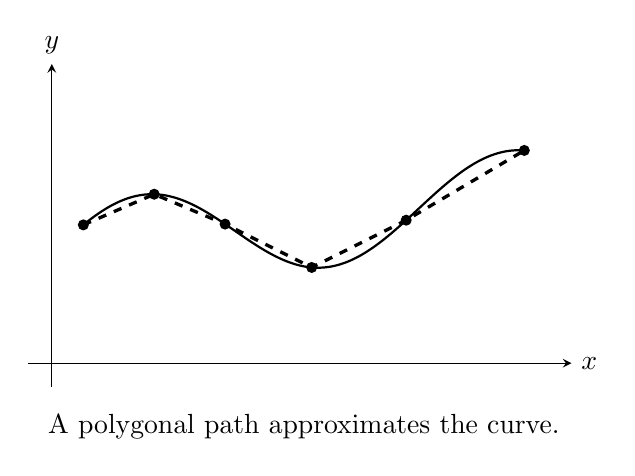
\begin{tikzpicture}[scale=1.0, >=stealth]
    \draw[->] (-0.3,0) -- (6.6,0) node[right] {\(x\)};
    \draw[->] (0,-0.3) -- (0,3.8) node[above] {\(y\)};

    \draw[thick, domain=0.4:6.0, samples=150, smooth, variable=\x]
        plot ({\x}, {1.4 + 0.6*sin(1.35*\x r) + 0.12*\x});

    \coordinate (P0) at (0.4,{1.4 + 0.6*sin(1.35*0.4 r) + 0.12*0.4});
    \coordinate (P1) at (1.3,{1.4 + 0.6*sin(1.35*1.3 r) + 0.12*1.3});
    \coordinate (P2) at (2.2,{1.4 + 0.6*sin(1.35*2.2 r) + 0.12*2.2});
    \coordinate (P3) at (3.3,{1.4 + 0.6*sin(1.35*3.3 r) + 0.12*3.3});
    \coordinate (P4) at (4.5,{1.4 + 0.6*sin(1.35*4.5 r) + 0.12*4.5});
    \coordinate (P5) at (6.0,{1.4 + 0.6*sin(1.35*6.0 r) + 0.12*6.0});

    \draw[very thick, dashed] (P0) -- (P1) -- (P2) -- (P3) -- (P4) -- (P5);

    \foreach \P in {P0,P1,P2,P3,P4,P5}
        \fill (\P) circle (2pt);

    \node at (3.2,-0.8) {A polygonal path approximates the curve.};
\end{tikzpicture}
\caption{Arc length is the limit of polygonal lengths.}
\end{figure}

On a small interval
\[
    [t_{i-1},t_i],
\]
the displacement is approximately
\[
    \mathbf r'(t_i^*)\Delta t_i
\]
for some point \(t_i^*\) in the interval.  Its length is approximately
\[
    \|\mathbf r'(t_i^*)\|\Delta t_i.
\]
So the polygonal length is approximately
\[
    \sum_{i=1}^N \|\mathbf r'(t_i^*)\|\Delta t_i.
\]
As the partition gets finer, this Riemann sum becomes
\[
    \int_a^b \|\mathbf r'(t)\|\,dt.
\]

\begin{theorem}[Arc length formula]
Let
\[
    \mathbf r:[a,b]\to\mathbb R^n
\]
be continuously differentiable.  Then the arc length of the curve is
\[
\boxed{
    L=\int_a^b \|\mathbf r'(t)\|\,dt.
}
\]
If the curve is only piecewise continuously differentiable, the same formula holds by
splitting the interval into smooth pieces and adding the lengths.
\end{theorem}

\begin{proof}[Proof idea]
On a very short interval, a differentiable curve is well approximated by its tangent line:
\[
    \mathbf r(t+\Delta t)-\mathbf r(t)
    \approx
    \mathbf r'(t)\Delta t.
\]
Taking lengths gives
\[
    \|\mathbf r(t+\Delta t)-\mathbf r(t)\|
    \approx
    \|\mathbf r'(t)\|\Delta t.
\]
Adding these approximations over the whole interval gives a Riemann sum for
\[
    \int_a^b \|\mathbf r'(t)\|\,dt.
\]
The continuity of \(\mathbf r'\) makes the approximation behave uniformly as the
subintervals shrink.
\end{proof}

The smoothness condition is there to keep the tangent approximation honest.

\begin{example}[A corner must be treated piece by piece]
Let
\[
    \mathbf r(t)=(|t|,t),
    \qquad -1\le t\le1.
\]
This curve has a corner at \(t=0\).  It is not differentiable there.

For \(t<0\),
\[
    \mathbf r(t)=(-t,t),
\]
so
\[
    \mathbf r'(t)=(-1,1),
    \qquad
    \|\mathbf r'(t)\|=\sqrt2.
\]
For \(t>0\),
\[
    \mathbf r(t)=(t,t),
\]
so
\[
    \mathbf r'(t)=(1,1),
    \qquad
    \|\mathbf r'(t)\|=\sqrt2.
\]
The curve is made of two straight segments, each of length \(\sqrt2\).  Therefore
\[
    L=2\sqrt2.
\]

We could not apply the smooth theorem on the whole interval at once, because the
velocity does not exist at \(t=0\).  But the curve is piecewise smooth, so we split it:
\[
    L
    =
    \int_{-1}^0\sqrt2\,dt
    +
    \int_0^1\sqrt2\,dt
    =
    2\sqrt2.
\]
The moral is simple: one corner is not a disaster, but it must be acknowledged.
\end{example}

\subsection{Arc length does not depend on the clock}

The same path can be traced slowly or quickly.  Its length should not change.

Consider the unit circle traced once:
\[
    \mathbf r_1(t)=(\cos t,\sin t),
    \qquad 0\le t\le2\pi.
\]
Its speed is
\[
    \|\mathbf r_1'(t)\|
    =
    \|(-\sin t,\cos t)\|
    =
    1.
\]
So its length is
\[
    L_1=\int_0^{2\pi}1\,dt=2\pi.
\]

Now trace the same circle using the slower clock
\[
    \mathbf r_2(u)=(\cos(2u),\sin(2u)),
    \qquad 0\le u\le\pi.
\]
This also goes once around the circle.  Its velocity is
\[
    \mathbf r_2'(u)=(-2\sin(2u),2\cos(2u)),
\]
and its speed is
\[
    \|\mathbf r_2'(u)\|=2.
\]
So
\[
    L_2=\int_0^\pi 2\,du=2\pi.
\]
The second clock runs over a shorter interval, but the speed with respect to that clock
is larger.  The product gives the same length.

This is the reason arc length is geometric.  It belongs to the curve, not to a particular
clock.

\subsection{The unit tangent vector}

Velocity gives both speed and direction.  If we want only the direction of motion, we
divide by the speed.

For the circle
\[
    \mathbf r(t)=(50\cos t,50\sin t),
\]
the velocity is
\[
    \mathbf r'(t)=(-50\sin t,50\cos t).
\]
The speed is
\[
    \|\mathbf r'(t)\|=50.
\]
So the direction of motion is
\[
    \frac{\mathbf r'(t)}{\|\mathbf r'(t)\|}
    =
    (-\sin t,\cos t).
\]
This vector has length \(1\), and it is tangent to the circle.

\begin{definition}[Unit tangent vector]
If
\[
    \mathbf r'(t)\ne\mathbf 0,
\]
then the \emph{unit tangent vector} is
\[
\boxed{
    \mathbf T(t)=\frac{\mathbf r'(t)}{\|\mathbf r'(t)\|}.
}
\]
It is the unit vector pointing in the direction of motion.
\end{definition}

The condition
\[
    \mathbf r'(t)\ne\mathbf 0
\]
matters.  If the velocity vector is zero, then there is no direction to divide by.

\begin{example}[A stopped particle has no unit tangent at that instant]
Let
\[
    \mathbf r(t)=(t^2,0),
    \qquad -1\le t\le1.
\]
This point moves left along the \(x\)-axis until \(t=0\), stops, and then moves right
along the same line.

The velocity is
\[
    \mathbf r'(t)=(2t,0).
\]
For \(t<0\),
\[
    \mathbf T(t)=(-1,0).
\]
For \(t>0\),
\[
    \mathbf T(t)=(1,0).
\]
At \(t=0\),
\[
    \mathbf r'(0)=(0,0),
\]
so
\[
    \frac{\mathbf r'(0)}{\|\mathbf r'(0)\|}
\]
is meaningless.

The geometric path is only the \(x\)-axis, but the moving point stops and reverses.
There is no single direction of motion at the stopping time.
\end{example}

A curve with
\[
    \mathbf r'(t)\ne\mathbf 0
\]
is often called \emph{regular}.  Regular curves do not stop.  They may turn, but they
always have a well-defined direction of motion.

\subsection{Reparametrization by arc length}

Sometimes the clock \(t\) is inconvenient.  A curve may speed up and slow down even
when its shape is simple.  Arc length gives a more geometric parameter.

Let
\[
    \mathbf r(t)=(2\cos t,2\sin t),
    \qquad 0\le t\le2\pi.
\]
The speed is
\[
    \|\mathbf r'(t)\|=2.
\]
The distance traveled from \(0\) to \(t\) is
\[
    s(t)=\int_0^t 2\,du=2t.
\]
So
\[
    t=\frac{s}{2}.
\]
Substituting into the curve gives
\[
    \mathbf R(s)=\mathbf r\left(\frac{s}{2}\right)
    =
    \left(2\cos\frac{s}{2},2\sin\frac{s}{2}\right),
    \qquad 0\le s\le4\pi.
\]
Now \(s\) measures distance traveled along the circle.  Differentiate:
\[
    \mathbf R'(s)=
    \left(
        -\sin\frac{s}{2},
        \cos\frac{s}{2}
    \right).
\]
Thus
\[
    \|\mathbf R'(s)\|=1.
\]
The curve is now traveled at unit speed.

\begin{definition}[Arc length function]
For a differentiable curve
\[
    \mathbf r:[a,b]\to\mathbb R^n,
\]
the \emph{arc length function} starting at \(a\) is
\[
\boxed{
    s(t)=\int_a^t \|\mathbf r'(u)\|\,du.
}
\]
It measures the distance traveled from time \(a\) to time \(t\).
\end{definition}

By the single-variable Fundamental Theorem of Calculus,
\[
    \frac{ds}{dt}=\|\mathbf r'(t)\|.
\]
So \(s\) increases at the speed of the moving point.

\begin{theorem}[Reparametrization by arc length]
Suppose
\[
    \mathbf r:[a,b]\to\mathbb R^n
\]
is continuously differentiable and
\[
    \|\mathbf r'(t)\|>0
\]
for all \(t\in[a,b]\).  Define
\[
    s(t)=\int_a^t \|\mathbf r'(u)\|\,du.
\]
Then \(s(t)\) is strictly increasing, so it has an inverse \(t=t(s)\).  The
reparametrized curve
\[
    \mathbf R(s)=\mathbf r(t(s))
\]
has unit speed:
\[
\boxed{
    \left\|\frac{d\mathbf R}{ds}\right\|=1.
}
\]
\end{theorem}

\begin{proof}
Since
\[
    \frac{ds}{dt}=\|\mathbf r'(t)\|>0,
\]
the function \(s(t)\) is strictly increasing and therefore invertible.

Using the chain rule,
\[
    \frac{d\mathbf R}{ds}
    =
    \frac{d\mathbf r}{dt}\frac{dt}{ds}.
\]
But
\[
    \frac{dt}{ds}
    =
    \frac{1}{ds/dt}
    =
    \frac{1}{\|\mathbf r'(t)\|}.
\]
Therefore
\[
    \frac{d\mathbf R}{ds}
    =
    \frac{\mathbf r'(t)}{\|\mathbf r'(t)\|}
    =
    \mathbf T(t).
\]
Taking lengths gives
\[
    \left\|\frac{d\mathbf R}{ds}\right\|=1.
\]
\end{proof}

The assumption
\[
    \|\mathbf r'(t)\|>0
\]
is not decoration.  If the curve stops for a while, arc length cannot serve as a clock.

\begin{example}[If the particle waits, arc length cannot recover the time]
Define a path on \(0\le t\le2\) by
\[
    \mathbf r(t)=
    \begin{cases}
    (0,0), & 0\le t\le1,\\
    (t-1,0), & 1\le t\le2.
    \end{cases}
\]
The point waits at the origin for one second, then moves to the right.

During the waiting time,
\[
    \|\mathbf r'(t)\|=0.
\]
So
\[
    s(t)=0
\]
for every \(0\le t\le1\).  The arc length function is not one-to-one.  Knowing
\[
    s=0
\]
does not tell us whether
\[
    t=0.2,\quad t=0.7,\quad \text{or}\quad t=1.
\]
So \(t\) cannot be recovered from \(s\).  Arc length is a good parameter only when the
motion never stalls.
\end{example}

Arc length solves the first problem raised by motion: how far did the point travel?
But it does not tell us how the curve bends.  Two roads can have the same length while
one is nearly straight and the other twists through sharp turns.  The unit tangent vector
\(\mathbf T\) records direction; the next question is how quickly that direction changes
as we move along the curve.  That rate of turning is called \emph{curvature}.

\section{Curvature and normal direction}
\label{sec:5.4}

Arc length gave us a fair way to measure progress along a curve.  It removed the
arbitrary clock.  Now we can ask a geometric question:

\[
    \text{How much does the curve turn per meter traveled?}
\]

That question leads to curvature.

\subsection{How sharply a curve turns}

A bicycle moving around a small traffic circle must turn sharply.  A bicycle moving
around a large roundabout turns gently.  Both paths are circles, but their radii are
different.

Start with a circle of radius \(R\):
\[
    \mathbf r(t)=(R\cos t,R\sin t).
\]
Its velocity is
\[
    \mathbf r'(t)=(-R\sin t,R\cos t),
\]
and its speed is
\[
    \|\mathbf r'(t)\|=R.
\]
The unit tangent vector is
\[
    \mathbf T(t)
    =
    \frac{\mathbf r'(t)}{\|\mathbf r'(t)\|}
    =
    (-\sin t,\cos t).
\]
Differentiate:
\[
    \mathbf T'(t)=(-\cos t,-\sin t).
\]
The length of this derivative is
\[
    \|\mathbf T'(t)\|=1.
\]

But this is the rate of change of \(\mathbf T\) with respect to \(t\), not with respect to
distance.  Since
\[
    \frac{ds}{dt}=R,
\]
we have
\[
    \frac{d\mathbf T}{ds}
    =
    \frac{d\mathbf T/dt}{ds/dt}
    =
    \frac{\mathbf T'(t)}{R}.
\]
Therefore
\[
    \left\|\frac{d\mathbf T}{ds}\right\|
    =
    \frac1R.
\]

A circle of radius \(R\) has curvature
\[
    \frac1R.
\]
Small radius means large curvature.  Large radius means small curvature.

\begin{figure}[h]
\centering
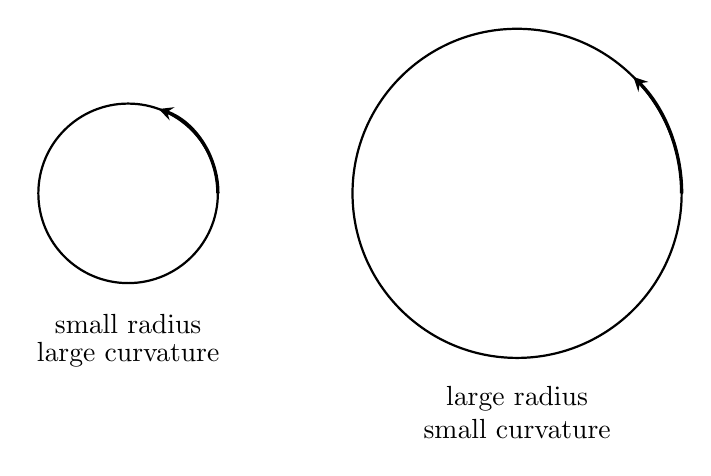
\begin{tikzpicture}[scale=0.95, >=stealth]
    \begin{scope}
        \draw[thick] (0,0) circle (1.2);
        \draw[->, very thick] (1.2,0) arc[start angle=0,end angle=70,radius=1.2];
        \node at (0,-1.75) {small radius};
        \node at (0,-2.15) {large curvature};
    \end{scope}

    \begin{scope}[shift={(5.2,0)}]
        \draw[thick] (0,0) circle (2.2);
        \draw[->, very thick] (2.2,0) arc[start angle=0,end angle=45,radius=2.2];
        \node at (0,-2.75) {large radius};
        \node at (0,-3.15) {small curvature};
    \end{scope}
\end{tikzpicture}
\caption{Curvature measures turning per unit distance, not turning per unit time.}
\end{figure}

This example tells us what the definition should be.

\begin{definition}[Curvature]
For a regular curve, the \emph{curvature} is
\[
\boxed{
    \kappa=\left\|\frac{d\mathbf T}{ds}\right\|.
}
\]
It measures how quickly the unit tangent vector changes per unit distance traveled.
\end{definition}

The letter \(\kappa\) is the Greek letter kappa.

Curvature has units of
\[
    \frac{1}{\text{length}}.
\]
For example, a circle of radius \(50\) meters has curvature
\[
    \frac{1}{50}\text{ per meter}.
\]

\subsection{Computing curvature from any parameter}

Curvature is defined using arc length \(s\), but most curves are given with some other
parameter \(t\).  The chain rule converts between them.

Since
\[
    \frac{ds}{dt}=\|\mathbf r'(t)\|,
\]
we have
\[
    \frac{d\mathbf T}{ds}
    =
    \frac{d\mathbf T/dt}{ds/dt}
    =
    \frac{\mathbf T'(t)}{\|\mathbf r'(t)\|}.
\]
Therefore
\[
\boxed{
    \kappa(t)=\frac{\|\mathbf T'(t)\|}{\|\mathbf r'(t)\|}.
}
\]

\begin{theorem}[Curvature from a parameter]
Let
\[
    \mathbf r(t)
\]
be a \(C^2\) regular curve.  Then
\[
\boxed{
    \kappa(t)=\frac{\|\mathbf T'(t)\|}{\|\mathbf r'(t)\|},
}
\]
where
\[
    \mathbf T(t)=\frac{\mathbf r'(t)}{\|\mathbf r'(t)\|}.
\]
\end{theorem}

\begin{proof}
The definition is
\[
    \kappa=\left\|\frac{d\mathbf T}{ds}\right\|.
\]
By the chain rule,
\[
    \frac{d\mathbf T}{dt}
    =
    \frac{d\mathbf T}{ds}\frac{ds}{dt}.
\]
Since
\[
    \frac{ds}{dt}=\|\mathbf r'(t)\|,
\]
we get
\[
    \frac{d\mathbf T}{ds}
    =
    \frac{\mathbf T'(t)}{\|\mathbf r'(t)\|}.
\]
Taking lengths gives the formula.
\end{proof}

The word \emph{regular} is essential.  If
\[
    \mathbf r'(t)=\mathbf 0,
\]
then \(\mathbf T(t)\) is not defined.

\begin{example}[Curvature fails at a stopping time]
Let
\[
    \mathbf r(t)=(t^2,0).
\]
For \(t<0\), the unit tangent vector is
\[
    \mathbf T(t)=(-1,0).
\]
For \(t>0\), it is
\[
    \mathbf T(t)=(1,0).
\]
At \(t=0\), the velocity is zero:
\[
    \mathbf r'(0)=(0,0).
\]
So the unit tangent is undefined there, and the curvature formula cannot be used at
that instant.

The path lies on a straight line, but the parametrized motion stops and reverses.
The regularity condition prevents this kind of ambiguity.
\end{example}

\subsection{A useful plane formula}

For a plane curve
\[
    \mathbf r(t)=(x(t),y(t)),
\]
there is a compact curvature formula:
\[
\boxed{
    \kappa(t)=
    \frac{|x'(t)y''(t)-y'(t)x''(t)|}
    {\left((x'(t))^2+(y'(t))^2\right)^{3/2}}.
}
\]

This formula is easier to remember if we recognize the numerator as a signed area
measurement:
\[
    x'y''-y'x''
    =
    \det
    \begin{pmatrix}
    x' & x''\\
    y' & y''
    \end{pmatrix}.
\]
It measures the signed area of the parallelogram spanned by
\[
    \mathbf r'(t)
    \qquad\text{and}\qquad
    \mathbf r''(t).
\]
In the language that will later become differential forms, it is the same alternating
measurement behind
\[
    dx\wedge dy.
\]

\begin{example}[Curvature of a parabola]
Let
\[
    \mathbf r(t)=(t,t^2).
\]
Then
\[
    x(t)=t,\qquad y(t)=t^2.
\]
So
\[
    x'(t)=1,\qquad y'(t)=2t,
\]
and
\[
    x''(t)=0,\qquad y''(t)=2.
\]
The curvature is
\[
\begin{aligned}
    \kappa(t)
    &=
    \frac{|x'y''-y'x''|}
    {\left((x')^2+(y')^2\right)^{3/2}}\\
    &=
    \frac{|1\cdot2-(2t)\cdot0|}
    {\left(1+4t^2\right)^{3/2}}\\
    &=
    \frac{2}{(1+4t^2)^{3/2}}.
\end{aligned}
\]
At the vertex,
\[
    t=0,
\]
the curvature is
\[
    \kappa(0)=2.
\]
Farther away from the vertex, the denominator grows, so the curvature decreases.  The
parabola bends most sharply at its vertex.
\end{example}

The denominator in the curvature formula must not be zero.  That denominator is
\[
    \left((x')^2+(y')^2\right)^{3/2}
    =
    \|\mathbf r'(t)\|^3.
\]
So the plane formula has the same regularity requirement:
\[
    \mathbf r'(t)\ne\mathbf 0.
\]

\subsection{Unit normal vector in the plane}

The tangent vector tells us the direction of motion.  When the curve turns, the tangent
vector changes.  The direction in which \(\mathbf T\) changes is the normal direction.

For the circle
\[
    \mathbf r(t)=(R\cos t,R\sin t),
\]
we found
\[
    \mathbf T(t)=(-\sin t,\cos t).
\]
Then
\[
    \mathbf T'(t)=(-\cos t,-\sin t).
\]
This points inward, toward the center of the circle.  Its length is \(1\), so the unit
normal vector is
\[
    \mathbf N(t)=(-\cos t,-\sin t).
\]

\begin{definition}[Unit normal vector]
If
\[
    \mathbf T'(t)\ne\mathbf 0,
\]
then the \emph{unit normal vector} is
\[
\boxed{
    \mathbf N(t)=\frac{\mathbf T'(t)}{\|\mathbf T'(t)\|}.
}
\]
It points in the direction the curve is turning.
\end{definition}

For a plane curve, \(\mathbf T\) and \(\mathbf N\) are perpendicular.  To see why,
notice that
\[
    \mathbf T(t)\cdot\mathbf T(t)=1
\]
for all \(t\).  Differentiate:
\[
    2\mathbf T(t)\cdot\mathbf T'(t)=0.
\]
Thus
\[
    \mathbf T(t)\cdot\mathbf T'(t)=0.
\]
So \(\mathbf T'(t)\), and therefore \(\mathbf N(t)\), is perpendicular to
\(\mathbf T(t)\).

\begin{figure}[h]
\centering
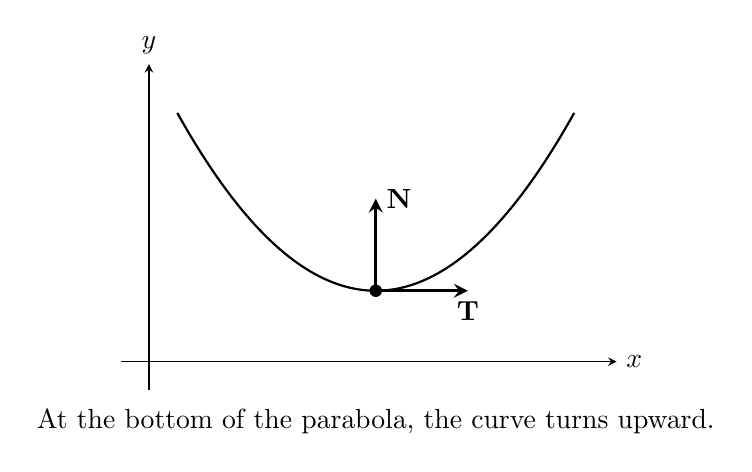
\begin{tikzpicture}[scale=0.9, >=stealth]
    \draw[->] (-0.4,0) -- (6.6,0) node[right] {\(x\)};
    \draw[->] (0,-0.4) -- (0,4.2) node[above] {\(y\)};

    \draw[thick, domain=0.4:6.0, samples=150, smooth, variable=\x]
        plot ({\x}, {1.0 + 0.32*(\x-3.2)^2});

    \coordinate (P) at (3.2,1.0);

    \fill (P) circle (2.5pt);
    \draw[->, very thick] (P) -- ++(1.3,0) node[below] {\(\mathbf T\)};
    \draw[->, very thick] (P) -- ++(0,1.3) node[right] {\(\mathbf N\)};

    \node at (3.2,-0.85) {At the bottom of the parabola, the curve turns upward.};
\end{tikzpicture}
\caption{The normal vector points toward the side where the tangent direction is changing.}
\end{figure}

The condition
\[
    \mathbf T'(t)\ne\mathbf 0
\]
also matters.

\begin{example}[A straight line has no preferred normal direction]
Let
\[
    \mathbf r(t)=(t,0).
\]
Then
\[
    \mathbf T(t)=(1,0)
\]
for every \(t\).  Therefore
\[
    \mathbf T'(t)=\mathbf 0.
\]
The curve is not turning, so there is no direction in which the tangent is changing.

Geometrically, the line has many perpendicular unit vectors, such as
\[
    (0,1)
    \qquad\text{and}\qquad
    (0,-1).
\]
But neither is chosen by the curve.  The normal vector \(\mathbf N\) is only defined
where the curve is actually turning.
\end{example}

When
\[
    \kappa>0,
\]
we can write
\[
\boxed{
    \frac{d\mathbf T}{ds}=\kappa\mathbf N.
}
\]
This is a compact way to read curvature and normal direction at once:
\[
    \text{change of tangent per unit length}
    =
    \text{amount of turning}\times\text{direction of turning}.
\]

\subsection{Curvature in space}

A space curve can bend without staying in one plane.  The definition of curvature does
not change:
\[
    \kappa=\left\|\frac{d\mathbf T}{ds}\right\|.
\]
The normal vector is still
\[
    \mathbf N=\frac{d\mathbf T/ds}{\|d\mathbf T/ds\|}
\]
when
\[
    \kappa>0.
\]

For computation in \(\mathbb R^3\), there is a useful formula involving the cross
product:
\[
\boxed{
    \kappa(t)=
    \frac{\|\mathbf r'(t)\times \mathbf r''(t)\|}
    {\|\mathbf r'(t)\|^3}.
}
\]

\begin{theorem}[Curvature formula in space]
Let
\[
    \mathbf r(t)
\]
be a \(C^2\) regular curve in \(\mathbb R^3\).  Then
\[
\boxed{
    \kappa(t)=
    \frac{\|\mathbf r'(t)\times \mathbf r''(t)\|}
    {\|\mathbf r'(t)\|^3}.
}
\]
\end{theorem}

\begin{proof}
Let
\[
    \sigma(t)=\|\mathbf r'(t)\|
\]
be the speed.  Then
\[
    \mathbf r'(t)=\sigma(t)\mathbf T(t).
\]
Differentiate:
\[
    \mathbf r''(t)=\sigma'(t)\mathbf T(t)+\sigma(t)\mathbf T'(t).
\]
Now take the cross product with \(\mathbf r'(t)=\sigma\mathbf T\):
\[
\begin{aligned}
    \mathbf r'\times\mathbf r''
    &=
    \sigma\mathbf T
    \times
    \bigl(\sigma'\mathbf T+\sigma\mathbf T'\bigr)\\
    &=
    \sigma\sigma'(\mathbf T\times\mathbf T)
    +
    \sigma^2(\mathbf T\times\mathbf T')\\
    &=
    \sigma^2(\mathbf T\times\mathbf T').
\end{aligned}
\]
Since
\[
    \mathbf T\cdot\mathbf T=1,
\]
we have
\[
    \mathbf T\cdot\mathbf T'=0.
\]
Thus \(\mathbf T\) and \(\mathbf T'\) are perpendicular, and \(\|\mathbf T\|=1\).  Hence
\[
    \|\mathbf T\times\mathbf T'\|=\|\mathbf T'\|.
\]
Therefore
\[
    \|\mathbf r'\times\mathbf r''\|
    =
    \sigma^2\|\mathbf T'\|.
\]
But
\[
    \kappa=\frac{\|\mathbf T'\|}{\|\mathbf r'\|}
    =
    \frac{\|\mathbf T'\|}{\sigma}.
\]
So
\[
    \|\mathbf T'\|=\kappa\sigma.
\]
Substitute:
\[
    \|\mathbf r'\times\mathbf r''\|
    =
    \sigma^2(\kappa\sigma)
    =
    \kappa\sigma^3.
\]
Therefore
\[
    \kappa=
    \frac{\|\mathbf r'\times\mathbf r''\|}{\|\mathbf r'\|^3}.
\]
\end{proof}

The hypothesis
\[
    \mathbf r'(t)\ne\mathbf 0
\]
again appears in the denominator.  A stopped particle has no unit tangent, so it has no
curvature as a parametrized motion at that instant.

\begin{example}[Curvature of a helix]
Let
\[
    \mathbf r(t)=(2\cos t,2\sin t,t).
\]
Then
\[
    \mathbf r'(t)=(-2\sin t,2\cos t,1),
\]
and
\[
    \mathbf r''(t)=(-2\cos t,-2\sin t,0).
\]
The speed is
\[
    \|\mathbf r'(t)\|
    =
    \sqrt{4\sin^2t+4\cos^2t+1}
    =
    \sqrt5.
\]
Compute the cross product:
\[
\begin{aligned}
    \mathbf r'(t)\times\mathbf r''(t)
    &=
    \begin{vmatrix}
    \mathbf i & \mathbf j & \mathbf k\\
    -2\sin t & 2\cos t & 1\\
    -2\cos t & -2\sin t & 0
    \end{vmatrix}\\
    &=
    (2\sin t,\;-2\cos t,\;4).
\end{aligned}
\]
Its length is
\[
    \sqrt{4\sin^2t+4\cos^2t+16}
    =
    \sqrt{20}
    =
    2\sqrt5.
\]
Therefore
\[
    \kappa(t)
    =
    \frac{2\sqrt5}{(\sqrt5)^3}
    =
    \frac{2}{5}.
\]
The curvature is constant.  A circular helix bends the same amount at every point.
\end{example}

A helix also twists out of its osculating plane, but that requires another measurement,
called torsion.  We will not need torsion in this course.  Curvature is the amount of
bending, and that is the part that controls normal acceleration.

\subsection{Tangential and normal components of acceleration}

Velocity can change in two different ways.

It can change length.  That means the object speeds up or slows down.

It can change direction.  That means the object turns.

Acceleration sees both.

Write the velocity as
\[
    \mathbf r'(t)=\sigma(t)\mathbf T(t),
\]
where
\[
    \sigma(t)=\|\mathbf r'(t)\|
\]
is speed.  Differentiate:
\[
\begin{aligned}
    \mathbf a(t)
    &=
    \mathbf r''(t)\\
    &=
    \sigma'(t)\mathbf T(t)+\sigma(t)\mathbf T'(t).
\end{aligned}
\]
Since
\[
    \frac{d\mathbf T}{ds}=\kappa\mathbf N
\]
and
\[
    \frac{ds}{dt}=\sigma,
\]
we get
\[
    \mathbf T'(t)
    =
    \frac{d\mathbf T}{ds}\frac{ds}{dt}
    =
    \kappa\mathbf N\,\sigma.
\]
Therefore
\[
\boxed{
    \mathbf a(t)=\sigma'(t)\mathbf T(t)+\kappa(t)\sigma(t)^2\mathbf N(t).
}
\]

This is one of the cleanest formulas in motion.

The first term,
\[
    \sigma'(t)\mathbf T(t),
\]
is tangential acceleration.  It changes speed.

The second term,
\[
    \kappa(t)\sigma(t)^2\mathbf N(t),
\]
is normal acceleration.  It changes direction.

\begin{definition}[Tangential and normal acceleration]
For a regular curve with speed
\[
    \sigma(t)=\|\mathbf r'(t)\|,
\]
the tangential component of acceleration is
\[
\boxed{
    a_T=\sigma'(t).
}
\]
The normal component of acceleration is
\[
\boxed{
    a_N=\kappa(t)\sigma(t)^2.
}
\]
Thus
\[
\boxed{
    \mathbf a=a_T\mathbf T+a_N\mathbf N.
}
\]
\end{definition}

The formula says something physical.  Turning at high speed requires large normal
acceleration because the speed is squared:
\[
    a_N=\kappa\sigma^2.
\]
This is why taking a sharp curve too fast is dangerous.

\begin{example}[A car on a circular track]
A car moves around a circular track of radius \(30\) meters at constant speed
\[
    12\text{ m/s}.
\]
The curvature of the track is
\[
    \kappa=\frac{1}{30}.
\]
Because the speed is constant,
\[
    a_T=0.
\]
The normal acceleration is
\[
    a_N=\kappa\sigma^2
    =
    \frac{1}{30}(12)^2
    =
    \frac{144}{30}
    =
    4.8.
\]
So the acceleration has magnitude
\[
    4.8\text{ m/s}^2
\]
and points inward, toward the center of the track.

The car is not speeding up, but it is accelerating because its direction is changing.
\end{example}

\begin{example}[Acceleration on a helix]
For
\[
    \mathbf r(t)=(2\cos t,2\sin t,t),
\]
we found
\[
    \sigma=\sqrt5,
    \qquad
    \kappa=\frac25.
\]
The speed is constant, so
\[
    a_T=\sigma'=0.
\]
The normal acceleration is
\[
    a_N=\kappa\sigma^2
    =
    \frac25\cdot5
    =
    2.
\]
Directly,
\[
    \mathbf r''(t)=(-2\cos t,-2\sin t,0),
\]
whose length is
\[
    2.
\]
So all of the acceleration is normal.  The moving point is not speeding up or slowing
down; it is being pulled toward the axis of the helix.
\end{example}

There is also a useful dot-product formula for the tangential component.  Since
\[
    \mathbf v=\sigma\mathbf T,
\]
we have
\[
    \mathbf v\cdot\mathbf a
    =
    \sigma\mathbf T\cdot(a_T\mathbf T+a_N\mathbf N).
\]
Because
\[
    \mathbf T\cdot\mathbf T=1
    \qquad\text{and}\qquad
    \mathbf T\cdot\mathbf N=0,
\]
this gives
\[
    \mathbf v\cdot\mathbf a=\sigma a_T.
\]
Therefore
\[
\boxed{
    a_T=\frac{\mathbf r'(t)\cdot\mathbf r''(t)}{\|\mathbf r'(t)\|}.
}
\]
In space, the normal component can be computed from
\[
\boxed{
    a_N=
    \frac{\|\mathbf r'(t)\times\mathbf r''(t)\|}{\|\mathbf r'(t)\|}.
}
\]
This follows from
\[
    a_N=\kappa\sigma^2
\]
and
\[
    \kappa=
    \frac{\|\mathbf r'\times\mathbf r''\|}{\|\mathbf r'\|^3}.
\]

\begin{example}[A path with both kinds of acceleration]
Let
\[
    \mathbf r(t)=(t,t^2),
    \qquad t>0.
\]
Then
\[
    \mathbf r'(t)=(1,2t),
    \qquad
    \mathbf r''(t)=(0,2).
\]
The speed is
\[
    \sigma(t)=\sqrt{1+4t^2}.
\]
So
\[
    a_T=\sigma'(t)=\frac{4t}{\sqrt{1+4t^2}}.
\]
The curvature of this parabola is
\[
    \kappa(t)=\frac{2}{(1+4t^2)^{3/2}}.
\]
Thus
\[
    a_N=\kappa\sigma^2
    =
    \frac{2}{(1+4t^2)^{3/2}}(1+4t^2)
    =
    \frac{2}{\sqrt{1+4t^2}}.
\]
The acceleration vector
\[
    \mathbf r''(t)=(0,2)
\]
has a tangential part and a normal part.  Part of it makes the point move faster; part
of it bends the motion upward.
\end{example}

This decomposition is useful because it separates two effects that are mixed together
inside the raw vector
\[
    \mathbf a=\mathbf r''.
\]

Curvature tells us how a path bends.  Tangential and normal acceleration tell us how
motion responds to that bending.  But some paths are better described not by
\(x,y,z\), but by radius and angle.  Circular motion, spirals, and planetary motion keep
asking for the same language: distance from a center, direction from a center, and the
area swept out by a moving radius.  That is where special coordinate systems begin to
pay back the work we spent learning them.
% =====================================================================
%  Chapter 5: Vector-Valed Functions and Motion
%  Sections 5.5 and 5.6
%  Project instructions and TOC consulted for continuity, forms thread,
%  and chapter structure. :contentReference[oaicite:0]{index=0} :contentReference[oaicite:1]{index=1}
%  Standard topic alignment cross-checked against common calculus texts.
%  :contentReference[oaicite:2]{index=2} :contentReference[oaicite:3]{index=3} :contentReference[oaicite:4]{index=4} :contentReference[oaicite:5]{index=5}
% =====================================================================

\section{Motion in special coordinate systems}
\label{sec:5.5}

Section \ref{sec:5.4} separated acceleration into two parts: one part changes speed,
and one part changes direction.  That was a geometric description.  Now we return to
the coordinate systems from Chapter 4 and ask how they describe the same motion.

Rectangular coordinates are not always the friendliest language.  A boat tracked by
radar is naturally described by distance and angle.  A planet moving around the sun is
naturally described by distance from the sun and angle swept around it.  For such
motions, polar coordinates do not merely shorten formulas.  They reveal structure.

\subsection{Velocity in polar coordinates}

A rescue boat leaves a harbor at sunset.  Its radar position is recorded by
\[
    r(t)=4+t,
    \qquad
    \theta(t)=\frac{t}{2},
\]
where \(r\) is measured in kilometers and \(t\) is measured in hours.  The boat is
moving outward because
\[
    r'(t)=1.
\]
It is also turning counterclockwise because
\[
    \theta'(t)=\frac12.
\]

At time \(t\), an increase in \(r\) moves the boat directly away from the harbor.  An
increase in \(\theta\) moves the boat sideways along a circle centered at the harbor.

At \(t=0\),
\[
    r=4.
\]
The radial speed is
\[
    r'=1.
\]
The sideways speed is not just \(\theta'\).  An angular change of \(\theta'\) radians per
hour along a circle of radius \(r\) gives tangential speed
\[
    r\theta'=4\cdot\frac12=2.
\]
So at \(t=0\), the velocity is made from two perpendicular pieces:
\[
    \text{radial part } 1,
    \qquad
    \text{angular part } 2.
\]
The speed is therefore
\[
    \sqrt{1^2+2^2}=\sqrt5.
\]

At \(t=2\),
\[
    r=6.
\]
The radial speed is still \(1\), but the sideways speed is now
\[
    r\theta'=6\cdot\frac12=3.
\]
So the speed is
\[
    \sqrt{1^2+3^2}=\sqrt{10}.
\]
The angular rate stayed the same, but the boat was farther from the center, so the
sideways motion became faster.

This example already contains the polar velocity formula.

To write it cleanly, define two unit vectors that move with the point:
\[
\boxed{
    \mathbf e_r=(\cos\theta,\sin\theta),
    \qquad
    \mathbf e_\theta=(-\sin\theta,\cos\theta).
}
\]
The vector \(\mathbf e_r\) points outward from the origin.  The vector \(\mathbf e_\theta\)
points in the direction of increasing angle.

\begin{figure}[h]
\centering
\begin{tikzpicture}[scale=0.95, >=stealth]
    \draw[->] (-0.5,0) -- (5.5,0) node[right] {\(x\)};
    \draw[->] (0,-0.5) -- (0,4.5) node[above] {\(y\)};

    \coordinate (O) at (0,0);
    \coordinate (P) at ({4*cos(35)}, {4*sin(35)});

    \draw[gray!35] (O) circle (4);
    \draw[->, thick] (O) -- (P) node[midway, below right] {\(r\)};

    \draw[thick] (1.1,0) arc[start angle=0,end angle=35,radius=1.1];
    \node at (1.45,0.35) {\(\theta\)};

    \fill (P) circle (2.5pt);

    \draw[->, very thick] (P) -- ++({1.2*cos(35)}, {1.2*sin(35)})
        node[above right] {\(\mathbf e_r\)};
    \draw[->, very thick] (P) -- ++({-1.2*sin(35)}, {1.2*cos(35)})
        node[above left] {\(\mathbf e_\theta\)};

    \node at (2.6,-1.0) {The polar unit vectors move with the point.};
\end{tikzpicture}
\caption{The unit vector \(\mathbf e_r\) points outward, and \(\mathbf e_\theta\) points
in the direction of increasing angle.}
\end{figure}

The position vector is
\[
    \mathbf R(t)=r(t)\mathbf e_r(t).
\]
Here \(\mathbf R\) is the actual position vector, while \(r(t)\) is the scalar distance from
the origin.

As \(\theta\) changes, the polar unit vectors rotate.  Differentiating
\[
    \mathbf e_r=(\cos\theta,\sin\theta)
\]
gives
\[
    \frac{d\mathbf e_r}{dt}
    =
    \theta'(-\sin\theta,\cos\theta)
    =
    \theta'\mathbf e_\theta.
\]
Similarly,
\[
    \frac{d\mathbf e_\theta}{dt}
    =
    -\theta'\mathbf e_r.
\]

Now differentiate the position:
\[
\begin{aligned}
    \mathbf v
    &=
    \frac{d}{dt}\bigl(r\mathbf e_r\bigr)\\
    &=
    r'\mathbf e_r+r\frac{d\mathbf e_r}{dt}\\
    &=
    r'\mathbf e_r+r\theta'\mathbf e_\theta.
\end{aligned}
\]

\begin{theorem}[Velocity in polar coordinates]
Suppose a plane motion is written in polar form as
\[
    \mathbf R(t)=r(t)\mathbf e_r(t),
\]
where \(r(t)\) and \(\theta(t)\) are differentiable.  Then
\[
\boxed{
    \mathbf v(t)=r'(t)\mathbf e_r+r(t)\theta'(t)\mathbf e_\theta.
}
\]
The speed is
\[
\boxed{
    \|\mathbf v(t)\|=
    \sqrt{(r'(t))^2+\bigl(r(t)\theta'(t)\bigr)^2}.
}
\]
\end{theorem}

\begin{proof}
The first formula follows from the product rule:
\[
    \frac{d}{dt}\bigl(r\mathbf e_r\bigr)
    =
    r'\mathbf e_r+r\mathbf e_r'.
\]
Since
\[
    \mathbf e_r'=\theta'\mathbf e_\theta,
\]
we get
\[
    \mathbf v=r'\mathbf e_r+r\theta'\mathbf e_\theta.
\]
The vectors \(\mathbf e_r\) and \(\mathbf e_\theta\) are perpendicular unit vectors, so
the length of the velocity is found by the Pythagorean theorem:
\[
    \|\mathbf v\|=\sqrt{(r')^2+(r\theta')^2}.
\]
\end{proof}

The hypotheses matter.  We need \(r(t)\) and \(\theta(t)\) to be differentiable, and we
need a polar description that behaves well.  The origin is a special danger point.

\begin{example}[The origin has no preferred angle]
The motion
\[
    \mathbf R(t)=(0,0)
\]
for all \(t\) is perfectly still.  Its velocity is
\[
    \mathbf v(t)=\mathbf 0.
\]
But in polar coordinates this same motion can be written as
\[
    r(t)=0,
    \qquad
    \theta(t)=t^2,
\]
or
\[
    r(t)=0,
    \qquad
    \theta(t)=\sin\frac1t
\]
for \(t\ne0\), or with almost any other angle function.  The angle does not describe
anything real when \(r=0\).

So polar formulas must be used with care at the origin.  A point at the origin has no
well-defined radial direction and no well-defined angular direction.
\end{example}

There is a second warning.  A geometric path may be smooth while a bad polar
description is not.

\begin{example}[A bad polar clock can create a fake problem]
The line motion
\[
    \mathbf R(t)=(t,0)
\]
is smooth.  Its velocity is
\[
    \mathbf R'(t)=(1,0)
\]
for every \(t\).

If we insist on \(r(t)\ge0\), then one polar description is
\[
    r(t)=|t|,
    \qquad
    \theta(t)=
    \begin{cases}
    \pi, & t<0,\\
    0, & t>0.
    \end{cases}
\]
At \(t=0\), this polar description has a corner in \(r\) and a jump in \(\theta\).  The
problem is not the original motion.  The problem is the polar coordinate description
at the origin.

Coordinates are tools.  At their singular points, they can misbehave.
\end{example}

\subsection{Acceleration in polar coordinates}

Velocity in polar coordinates has two pieces:
\[
    \mathbf v=r'\mathbf e_r+r\theta'\mathbf e_\theta.
\]
Acceleration comes from differentiating this formula.  Because the basis vectors
\(\mathbf e_r\) and \(\mathbf e_\theta\) rotate as the point moves, the result contains
more than just \(r''\) and \(\theta''\).

Differentiate:
\[
\begin{aligned}
    \mathbf a
    &=
    \frac{d}{dt}\left(r'\mathbf e_r+r\theta'\mathbf e_\theta\right)\\
    &=
    r''\mathbf e_r+r'\mathbf e_r'
    +(r'\theta'+r\theta'')\mathbf e_\theta
    +r\theta'\mathbf e_\theta'.
\end{aligned}
\]
Use
\[
    \mathbf e_r'=\theta'\mathbf e_\theta,
    \qquad
    \mathbf e_\theta'=-\theta'\mathbf e_r.
\]
Then
\[
\begin{aligned}
    \mathbf a
    &=
    r''\mathbf e_r
    +r'\theta'\mathbf e_\theta
    +(r'\theta'+r\theta'')\mathbf e_\theta
    -r(\theta')^2\mathbf e_r\\
    &=
    \bigl(r''-r(\theta')^2\bigr)\mathbf e_r
    +
    \bigl(r\theta''+2r'\theta'\bigr)\mathbf e_\theta.
\end{aligned}
\]

\begin{theorem}[Acceleration in polar coordinates]
Suppose
\[
    \mathbf R(t)=r(t)\mathbf e_r(t)
\]
is a plane motion with \(r(t)\) and \(\theta(t)\) twice differentiable.  Then
\[
\boxed{
    \mathbf a(t)
    =
    \bigl(r''-r(\theta')^2\bigr)\mathbf e_r
    +
    \bigl(r\theta''+2r'\theta'\bigr)\mathbf e_\theta.
}
\]
\end{theorem}

The twice differentiable condition is not decoration.  Acceleration is a second
derivative.  If the motion has a corner or a sudden reversal, the acceleration formula
has no honest value at that instant.

\begin{example}[A corner in angle destroys velocity at the corner]
Let
\[
    r(t)=1,
    \qquad
    \theta(t)=|t|.
\]
The position is
\[
    \mathbf R(t)=(\cos|t|,\sin|t|).
\]
For \(t>0\), the point moves counterclockwise on the unit circle.  For \(t<0\), it moves
clockwise.  At \(t=0\), the point is
\[
    (1,0),
\]
but the velocity from the left points downward while the velocity from the right points
upward.

So \(\mathbf R'(0)\) does not exist.  The formula for acceleration cannot be used at
\(t=0\).  The hypothesis that \(r\) and \(\theta\) are differentiable is doing real work.
\end{example}

\subsection{Circular motion and angular velocity}

Circular motion is the cleanest polar motion.  The radius is constant:
\[
    r(t)=R.
\]
The angle changes:
\[
    \theta=\theta(t).
\]
The angular velocity is
\[
\boxed{
    \omega(t)=\theta'(t).
}
\]

From the polar velocity formula,
\[
    \mathbf v=R\omega\,\mathbf e_\theta.
\]
So the speed is
\[
\boxed{
    \|\mathbf v\|=R|\omega|.
}
\]
A larger circle gives a larger speed for the same angular velocity.

The acceleration formula gives
\[
\boxed{
    \mathbf a=-R\omega^2\mathbf e_r+R\omega'\mathbf e_\theta.
}
\]
The radial term
\[
    -R\omega^2\mathbf e_r
\]
points inward.  The tangential term
\[
    R\omega'\mathbf e_\theta
\]
appears only when the angular velocity changes.

\begin{example}[A spinning observation wheel]
A seat on an observation wheel of radius \(20\) meters rotates with constant angular
velocity
\[
    \omega=\frac{\pi}{30}
\]
radians per second.  Its speed is
\[
    R|\omega|
    =
    20\cdot\frac{\pi}{30}
    =
    \frac{2\pi}{3}
\]
meters per second.

Since \(\omega\) is constant,
\[
    \omega'=0.
\]
So the acceleration is purely inward:
\[
    \mathbf a=-R\omega^2\mathbf e_r.
\]
Its magnitude is
\[
    R\omega^2
    =
    20\left(\frac{\pi}{30}\right)^2
    =
    \frac{\pi^2}{45}.
\]
The rider is not speeding up, but the rider is accelerating because the direction of
motion is continuously changing.
\end{example}

This agrees with Section \ref{sec:5.4}.  A circle of radius \(R\) has curvature
\[
    \kappa=\frac1R.
\]
The speed is
\[
    \sigma=R|\omega|.
\]
So the normal acceleration is
\[
    a_N=\kappa\sigma^2
    =
    \frac1R(R^2\omega^2)
    =
    R\omega^2.
\]
The same fact has appeared twice: once from curvature, and once from polar
coordinates.

\begin{example}[Circular motion that speeds up]
Let
\[
    r(t)=3,
    \qquad
    \theta(t)=t^2.
\]
Then
\[
    \omega(t)=2t,
    \qquad
    \omega'(t)=2.
\]
The velocity is
\[
    \mathbf v=3(2t)\mathbf e_\theta=6t\mathbf e_\theta.
\]
The acceleration is
\[
    \mathbf a
    =
    -3(2t)^2\mathbf e_r+3(2)\mathbf e_\theta
    =
    -12t^2\mathbf e_r+6\mathbf e_\theta.
\]
The inward part grows as \(t^2\), because the speed is increasing.  The tangential part
is constant, because the angular velocity increases at a constant rate.
\end{example}

\subsection{Planetary motion as a guiding example}

A planet moving around the sun is not usually best described by \(x(t)\) and \(y(t)\).
The natural questions are radial:

\[
    \text{How far from the sun?}
    \qquad
    \text{How fast is the radius vector turning?}
\]

Put the sun at the origin.  Suppose the planet has position
\[
    \mathbf R(t)=r(t)\mathbf e_r.
\]
Gravity pulls along the line from the planet to the sun.  That means the acceleration
has no \(\mathbf e_\theta\) component.  In polar coordinates,
\[
    \mathbf a
    =
    \bigl(r''-r(\theta')^2\bigr)\mathbf e_r
    +
    \bigl(r\theta''+2r'\theta'\bigr)\mathbf e_\theta.
\]
So a central force gives
\[
    r\theta''+2r'\theta'=0.
\]
Multiply by \(r\):
\[
    r^2\theta''+2rr'\theta'=0.
\]
But the left side is the derivative of
\[
    r^2\theta':
\]
indeed,
\[
    \frac{d}{dt}\bigl(r^2\theta'\bigr)
    =
    2rr'\theta'+r^2\theta''.
\]
Therefore
\[
\boxed{
    r^2\theta'=h
}
\]
for some constant \(h\).

This quantity is the angular momentum per unit mass.  It is also the key to a beautiful
area fact.

\subsection{The area swept out by a radius vector}

Imagine the planet at two nearby times.  The radius vector from the sun to the planet
sweeps out a thin wedge.  For a small angle change \(\Delta\theta\), the area is
approximately
\[
    \frac12 r^2\Delta\theta.
\]
So the rate at which area is swept should be
\[
    \frac12 r^2\theta'.
\]
The calculation above says this rate is constant for central-force motion.

\begin{figure}[h]
\centering
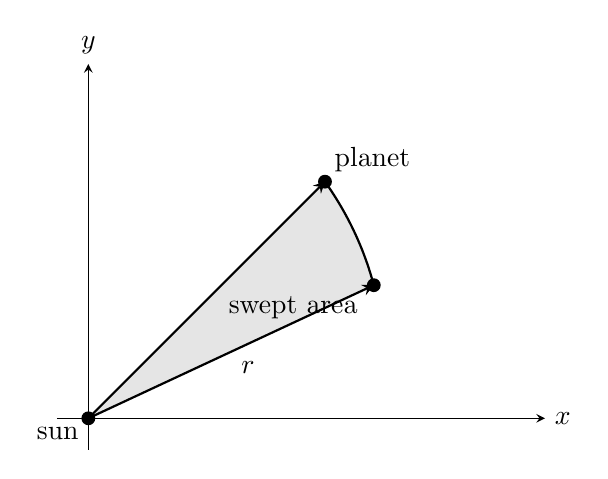
\begin{tikzpicture}[scale=1.0, >=stealth]
    \draw[->] (-0.4,0) -- (5.8,0) node[right] {\(x\)};
    \draw[->] (0,-0.4) -- (0,4.5) node[above] {\(y\)};

    \coordinate (O) at (0,0);
    \coordinate (P) at (25:4);
    \coordinate (Q) at (45:4.25);

    % Smoothly interpolate the radius from 4 to 4.25
    \fill[gray!20] (O) -- (P) 
        -- plot[domain=25:45, samples=30, variable=\t] 
            ({(4 + 0.0125*(\t-25)) * cos(\t)}, {(4 + 0.0125*(\t-25)) * sin(\t)}) 
        -- cycle;

    \draw[->, thick] (O) -- (P) node[midway, below right] {\(r\)};
    \draw[->, thick] (O) -- (Q);
    
    \draw[thick] plot[domain=25:45, samples=30, variable=\t] 
        ({(4 + 0.0125*(\t-25)) * cos(\t)}, {(4 + 0.0125*(\t-25)) * sin(\t)});

    \fill (O) circle (2.5pt);
    \fill (P) circle (2.5pt);
    \fill (Q) circle (2.5pt);

    \node[below left] at (O) {sun};
    \node[above right] at (Q) {planet};
    \node at (2.6,1.4) {swept area};
\end{tikzpicture}
\caption{A radius vector sweeps out area as the angle changes.}
\end{figure}

\begin{definition}[Signed swept area]
For a plane motion
\[
    \mathbf R(t)=(x(t),y(t)),
\]
the signed area swept out by the radius vector from time \(a\) to time \(b\) is
\[
\boxed{
    A=\frac12\int_a^b \bigl(x(t)y'(t)-y(t)x'(t)\bigr)\,dt.
}
\]
In polar coordinates this becomes
\[
\boxed{
    A=\frac12\int_a^b r(t)^2\theta'(t)\,dt.
}
\]
\end{definition}

Here is the polar calculation.  If
\[
    x=r\cos\theta,\qquad y=r\sin\theta,
\]
then
\[
    x\,dy-y\,dx=r^2\,d\theta.
\]
Along the curve,
\[
    d\theta=\theta'(t)\,dt.
\]
So
\[
    \frac12(x\,dy-y\,dx)
    =
    \frac12r^2\,d\theta
    =
    \frac12r^2\theta'(t)\,dt.
\]

This is our first clear appearance of a \(1\)-form that measures an area swept along a
curve:
\[
\boxed{
    \omega_A=\frac12(x\,dy-y\,dx).
}
\]
Later, line integrals will make this language systematic.  For now, it is enough to
notice the pattern: a small movement of a point can contribute a small signed area.

\begin{theorem}[Kepler's second law for central acceleration]
Suppose a plane motion satisfies
\[
    r(t)>0
\]
and has acceleration always parallel to \(\mathbf e_r\).  Then
\[
    r(t)^2\theta'(t)
\]
is constant.  Therefore the signed area swept out per unit time,
\[
\boxed{
    \frac{dA}{dt}=\frac12r(t)^2\theta'(t),
}
\]
is constant.

In words: equal time intervals sweep out equal signed areas.
\end{theorem}

\begin{proof}
If the acceleration is always radial, then its \(\mathbf e_\theta\)-component is zero:
\[
    r\theta''+2r'\theta'=0.
\]
Since \(r>0\), multiply by \(r\):
\[
    r^2\theta''+2rr'\theta'=0.
\]
But
\[
    \frac{d}{dt}(r^2\theta')
    =
    r^2\theta''+2rr'\theta'.
\]
So
\[
    \frac{d}{dt}(r^2\theta')=0.
\]
Thus
\[
    r^2\theta'
\]
is constant.  Since
\[
    \frac{dA}{dt}=\frac12r^2\theta',
\]
the swept area rate is also constant.
\end{proof}

The condition that the acceleration be radial is essential.

\begin{example}[Tangential acceleration breaks equal areas]
Let
\[
    r(t)=1,
    \qquad
    \theta(t)=t^2.
\]
Then
\[
    r^2\theta'=2t,
\]
which is not constant.  The signed swept area rate is
\[
    \frac{dA}{dt}=\frac12(2t)=t.
\]
The radius vector sweeps area faster as time passes.

The polar acceleration has \(\mathbf e_\theta\)-component
\[
    r\theta''+2r'\theta'=1\cdot2+0=2.
\]
So the acceleration is not purely radial.  There is tangential acceleration, and equal
areas in equal times fail.
\end{example}

There is also a warning about the word \emph{signed}.

\begin{example}[Signed swept area can cancel]
Let
\[
    r(t)=1,
    \qquad
    \theta(t)=\sin t,
    \qquad
    0\le t\le2\pi.
\]
Then
\[
    \theta'(t)=\cos t.
\]
The signed swept area is
\[
    A=\frac12\int_0^{2\pi}\cos t\,dt=0.
\]
But the radius vector did move.  It swept forward and then backward, and the signed
areas canceled.

So the formula
\[
    \frac12\int r^2\theta'\,dt
\]
measures signed swept area.  If a ray backtracks, total physical area swept may require
separating the intervals and adding absolute values.
\end{example}

Special coordinates have now done two things for us.  They shortened computations,
and they exposed hidden quantities: angular velocity, inward acceleration, and swept
area.  The chapter has one more job: gather the whole toolbox and see how it works in
larger motion problems, from projectiles with air resistance to the curvature of roads.

\section{Chapter review and applications}
\label{sec:5.6}

% Author's note: This section intentionally differs from the usual section anatomy.
% It is a chapter review, so it gathers formulas, worked review examples, and projects
% rather than introducing one new theorem.

Chapter 5 began with a moving point
\[
    \mathbf r(t).
\]
From that one object came velocity, acceleration, speed, arc length, curvature, normal
direction, polar motion, angular velocity, and swept area.  The point moved through a
curve, but the calculus happened through one variable: time.

\subsection{The formula map}

Here are the main tools of the chapter.

\[
\begin{array}{c|c}
\text{Idea} & \text{Formula} \\ \hline
\text{velocity} & \mathbf v(t)=\mathbf r'(t)\\[1mm]
\text{acceleration} & \mathbf a(t)=\mathbf r''(t)\\[1mm]
\text{speed} & \sigma(t)=\|\mathbf r'(t)\|\\[1mm]
\text{arc length} & L=\displaystyle\int_a^b \|\mathbf r'(t)\|\,dt\\[3mm]
\text{unit tangent} & \mathbf T(t)=\dfrac{\mathbf r'(t)}{\|\mathbf r'(t)\|}\\[4mm]
\text{curvature} & \kappa=\left\|\dfrac{d\mathbf T}{ds}\right\|\\[4mm]
\text{curvature from a parameter} &
\kappa(t)=\dfrac{\|\mathbf T'(t)\|}{\|\mathbf r'(t)\|}\\[4mm]
\text{space curvature formula} &
\kappa(t)=\dfrac{\|\mathbf r'(t)\times\mathbf r''(t)\|}{\|\mathbf r'(t)\|^3}\\[4mm]
\text{acceleration split} &
\mathbf a=a_T\mathbf T+a_N\mathbf N\\[1mm]
\text{tangential acceleration} & a_T=\sigma'(t)\\[1mm]
\text{normal acceleration} & a_N=\kappa\sigma^2\\[1mm]
\text{polar velocity} &
\mathbf v=r'\mathbf e_r+r\theta'\mathbf e_\theta\\[1mm]
\text{polar acceleration} &
\mathbf a=(r''-r(\theta')^2)\mathbf e_r+(r\theta''+2r'\theta')\mathbf e_\theta\\[1mm]
\text{signed swept area} &
A=\dfrac12\displaystyle\int_a^b (xy'-yx')\,dt
=\dfrac12\displaystyle\int_a^b r^2\theta'\,dt
\end{array}
\]

The formulas are less separate than they look.  The speed \(\sigma\) is the bridge from
time to distance:
\[
    ds=\sigma\,dt.
\]
Curvature measures how fast the tangent changes with respect to distance:
\[
    \kappa=\left\|\frac{d\mathbf T}{ds}\right\|.
\]
Polar coordinates split velocity into radial and angular pieces.  The swept-area form
\[
    \frac12(x\,dy-y\,dx)
\]
quietly points toward the next big subject: integrating forms along paths.

\subsection{A complete review example}

Consider the helix
\[
    \mathbf r(t)=(3\cos t,3\sin t,4t),
    \qquad 0\le t\le2\pi.
\]
This is one turn around a cylinder of radius \(3\), rising \(8\pi\) units in height.

First,
\[
    \mathbf r'(t)=(-3\sin t,3\cos t,4),
\]
so the speed is
\[
    \|\mathbf r'(t)\|
    =
    \sqrt{9\sin^2t+9\cos^2t+16}
    =
    5.
\]
The length of one turn is
\[
    L=\int_0^{2\pi}5\,dt=10\pi.
\]

The unit tangent vector is
\[
    \mathbf T(t)=\frac15(-3\sin t,3\cos t,4).
\]
Since the speed is constant, the tangential acceleration is
\[
    a_T=0.
\]
The acceleration is
\[
    \mathbf r''(t)=(-3\cos t,-3\sin t,0).
\]
Its length is
\[
    \|\mathbf r''(t)\|=3.
\]
Because the speed is constant, all acceleration is normal, so
\[
    a_N=3.
\]

Now compute curvature:
\[
    \mathbf r'(t)\times\mathbf r''(t)
    =
    (12\sin t,-12\cos t,9).
\]
Thus
\[
    \|\mathbf r'(t)\times\mathbf r''(t)\|
    =
    \sqrt{144\sin^2t+144\cos^2t+81}
    =
    15.
\]
Therefore
\[
    \kappa(t)=\frac{15}{5^3}=\frac{3}{25}.
\]
This agrees with
\[
    a_N=\kappa\sigma^2,
\]
because
\[
    \frac{3}{25}\cdot 25=3.
\]

The helix has constant speed and constant curvature.  It bends the same amount at
every point.

\subsection{Skill summary}

By the end of this chapter, a student should be able to do the following.

\begin{enumerate}
\item Read a vector-valued function as a moving point:
\[
    \mathbf r(t)=(x(t),y(t),z(t)).
\]

\item Differentiate and integrate component by component:
\[
    \mathbf r'(t)=(x'(t),y'(t),z'(t)),
\]
and
\[
    \int_a^b \mathbf v(t)\,dt
    =
    \left(
    \int_a^b v_1(t)\,dt,\int_a^b v_2(t)\,dt,\int_a^b v_3(t)\,dt
    \right).
\]

\item Find tangent lines:
\[
    \mathbf L(s)=\mathbf r(a)+s\mathbf r'(a),
\]
when
\[
    \mathbf r'(a)\ne\mathbf 0.
\]

\item Compute distance traveled:
\[
    L=\int_a^b \|\mathbf r'(t)\|\,dt.
\]

\item Reparametrize simple curves by arc length when the speed never vanishes.

\item Compute the unit tangent vector:
\[
    \mathbf T=\frac{\mathbf r'}{\|\mathbf r'\|}.
\]

\item Compute curvature in the plane or in space:
\[
    \kappa(t)=
    \frac{|x'y''-y'x''|}
    {\left((x')^2+(y')^2\right)^{3/2}}
\]
for plane curves, and
\[
    \kappa(t)=
    \frac{\|\mathbf r'\times\mathbf r''\|}
    {\|\mathbf r'\|^3}
\]
for space curves.

\item Split acceleration into tangential and normal parts:
\[
    \mathbf a=a_T\mathbf T+a_N\mathbf N,
\qquad
    a_T=\sigma',
\qquad
    a_N=\kappa\sigma^2.
\]

\item Use polar coordinates for motion:
\[
    \mathbf v=r'\mathbf e_r+r\theta'\mathbf e_\theta.
\]

\item Recognize the central-force area law:
\[
    \text{radial acceleration}
    \quad\Longrightarrow\quad
    r^2\theta'=\text{constant}
    \quad\Longrightarrow\quad
    \frac{dA}{dt}=\text{constant}.
\]
\end{enumerate}

\subsection{Project: projectile motion with air resistance}

Without air resistance, a projectile follows a parabola.  With air resistance, it does not.
But vector-valued functions still organize the motion.

Let the \(z\)-axis point upward.  A projectile has position
\[
    \mathbf r(t)=(x(t),y(t),z(t))
\]
and velocity
\[
    \mathbf v(t)=\mathbf r'(t).
\]
Assume gravity is
\[
    -g\mathbf k
\]
and air resistance is proportional to velocity:
\[
    -c\mathbf v.
\]
If the mass is \(m\), Newton's law gives
\[
    m\mathbf v'=-mg\mathbf k-c\mathbf v.
\]
Set
\[
    k=\frac{c}{m}.
\]
Then
\[
\boxed{
    \mathbf v'=-k\mathbf v-g\mathbf k.
}
\]

Suppose
\[
    \mathbf r(0)=(x_0,y_0,z_0)
\]
and
\[
    \mathbf v(0)=(v_{x0},v_{y0},v_{z0}).
\]
The velocity components are
\[
\boxed{
    v_x(t)=v_{x0}e^{-kt},
}
\]
\[
\boxed{
    v_y(t)=v_{y0}e^{-kt},
}
\]
and
\[
\boxed{
    v_z(t)=\left(v_{z0}+\frac{g}{k}\right)e^{-kt}-\frac{g}{k}.
}
\]
Integrating gives the position:
\[
\boxed{
    x(t)=x_0+\frac{v_{x0}}{k}\left(1-e^{-kt}\right),
}
\]
\[
\boxed{
    y(t)=y_0+\frac{v_{y0}}{k}\left(1-e^{-kt}\right),
}
\]
and
\[
\boxed{
    z(t)=
    z_0+
    \frac{v_{z0}+g/k}{k}\left(1-e^{-kt}\right)
    -\frac{g}{k}t.
}
\]

This project can be explored in stages.

\begin{enumerate}
\item Verify by differentiating that the formulas for \(v_x,v_y,v_z\) satisfy
\[
    \mathbf v'=-k\mathbf v-g\mathbf k.
\]

\item Verify by differentiating that the formulas for \(x,y,z\) satisfy
\[
    \mathbf r'(t)=\mathbf v(t).
\]

\item Choose numerical values, such as
\[
    g=9.8,\qquad k=0.15,\qquad
    \mathbf r(0)=(0,0,1),\qquad
    \mathbf v(0)=(20,0,18).
\]
Find the time when
\[
    z(t)=0.
\]
This equation usually needs numerical solving.

\item Compare the horizontal distance traveled with and without air resistance.

\item Plot the path
\[
    (x(t),z(t))
\]
in the vertical plane.  The no-drag path is a parabola.  The drag path is not.
\end{enumerate}

The point of the project is not that every motion has a simple formula.  The point is
that velocity and acceleration still give the right language, even when the path stops
looking like the clean parabolas from single-variable calculus.

\subsection{Project: curvature of a road or roller coaster track}

A road designer cares about curvature because curvature controls normal acceleration.
If a car moves with speed \(\sigma\) along a road of curvature \(\kappa\), then
\[
    a_N=\kappa\sigma^2.
\]
The speed is squared.  This is why doubling speed is not twice as demanding on a
curve; it is four times as demanding.

Suppose a road centerline in the plane is modeled by
\[
    y=f(x).
\]
A convenient parametrization is
\[
    \mathbf r(x)=(x,f(x)).
\]
Then
\[
    \mathbf r'(x)=(1,f'(x)),
\qquad
    \mathbf r''(x)=(0,f''(x)).
\]
The plane curvature formula becomes
\[
\boxed{
    \kappa(x)=
    \frac{|f''(x)|}{\left(1+(f'(x))^2\right)^{3/2}}.
}
\]

If the allowed normal acceleration is \(A\), then a safe speed should satisfy
\[
    \kappa\sigma^2\le A.
\]
So, where \(\kappa>0\),
\[
\boxed{
    \sigma\le \sqrt{\frac{A}{\kappa}}.
}
\]

\begin{example}[A simple speed estimate]
Suppose a road near its sharpest bend is modeled by
\[
    y=0.005x^2,
\]
where \(x\) and \(y\) are measured in meters.  Then
\[
    f'(x)=0.01x,
    \qquad
    f''(x)=0.01.
\]
At \(x=0\),
\[
    \kappa(0)=0.01.
\]
If a comfortable normal acceleration is
\[
    A=3\text{ m/s}^2,
\]
then
\[
    \sigma\le \sqrt{\frac{3}{0.01}}=\sqrt{300}\approx17.3\text{ m/s}.
\]
The curvature calculation has turned a geometric bend into a speed recommendation.
\end{example}

A fuller project can use real data.

\begin{enumerate}
\item Choose a road, bike path, running track, or roller coaster curve.

\item Model its centerline by a parametrized curve
\[
    \mathbf r(t)=(x(t),y(t))
\]
or
\[
    \mathbf r(t)=(x(t),y(t),z(t)).
\]

\item Compute or numerically estimate
\[
    \kappa(t).
\]

\item Find where the curvature is largest.

\item Use
\[
    a_N=\kappa\sigma^2
\]
to estimate a speed limit or a required banking design.

\item Explain the physical meaning of the largest curvature point.  Is it a tight turn,
a sudden vertical bend, or a combination?
\end{enumerate}

This project is a good test of the whole chapter.  The curve gives position.  The first
derivative gives direction and speed.  The second derivative reveals turning.  Curvature
turns that geometry into a physical constraint.

\subsection{Review problems}

\begin{enumerate}
\item For
\[
    \mathbf r(t)=(t,t^2,\ln t),
    \qquad t>0,
\]
find \(\mathbf v(t)\), \(\mathbf a(t)\), and the speed.

\item Find the tangent line to
\[
    \mathbf r(t)=(e^t,\cos t,\sin t)
\]
at \(t=0\).

\item Compute the length of
\[
    \mathbf r(t)=(4\cos t,4\sin t,3t),
    \qquad 0\le t\le2\pi.
\]

\item Find the unit tangent vector for
\[
    \mathbf r(t)=(t,t^2)
\]
at \(t=1\).

\item Compute the curvature of the parabola
\[
    \mathbf r(t)=(t,t^2)
\]
at \(t=0\) and at \(t=1\).  Where is the curve bending more sharply?

\item Let
\[
    \mathbf r(t)=(2\cos t,2\sin t,t).
\]
Find the speed, curvature, tangential acceleration, and normal acceleration.

\item For the polar motion
\[
    r(t)=1+t,
    \qquad
    \theta(t)=t^2,
\]
find the radial and angular components of velocity.

\item For the polar motion
\[
    r(t)=3,
    \qquad
    \theta(t)=t^3,
\]
find the radial and angular components of acceleration.

\item A point moves with
\[
    r^2\theta'=12.
\]
Find the signed area swept out from \(t=1\) to \(t=5\).

\item Show that if a motion has constant speed, then its acceleration is perpendicular
to its velocity.

\item A car moves at \(15\) m/s along a road with curvature \(0.02\).  Find its normal
acceleration.

\item A curve has speed \(4\) and curvature \(0.5\) at a certain instant.  Find the
normal component of acceleration at that instant.

\item Let
\[
    \mathbf r(t)=(t^2,t^3).
\]
Show that \(\mathbf r'(0)=\mathbf 0\).  What does this say about the unit tangent
formula at \(t=0\)?

\item Let
\[
    \mathbf r(t)=(\cos t,\sin t)
\]
for \(0\le t\le4\pi\).  What is the displacement?  What is the distance traveled?

\item Let
\[
    \omega_A=\frac12(x\,dy-y\,dx).
\]
For the circle
\[
    \mathbf r(t)=(R\cos t,R\sin t),
    \qquad 0\le t\le2\pi,
\]
compute
\[
    \int_{\mathbf r}\omega_A.
\]
What area does this recover?
\end{enumerate}

A curve has only one direction of travel at a time.  That made the derivative
\[
    \mathbf r'(t)
\]
a single vector.  A surface is different.  At a point on a sheet of paper, a hillside, or a
sphere, there are many possible directions to move.  The next chapter begins there:
not with motion along one path, but with functions whose inputs fill a region.  A
single slope number will no longer be enough.